\documentclass[10pt,t,english]{beamer}
\usepackage{fontawesome}
\usepackage{graphicx}
\usepackage{array}
\usepackage[normalem]{ulem}
\usepackage{amsfonts,amsmath,amssymb,bm,bbm}
\usepackage{mathrsfs}
\usepackage{sgame}
\usepackage{graphicx,pstricks}
\usepackage{xcolor}
\usepackage{colortbl}
\usepackage{makecell}
\usepackage{tikz,tikzsymbols,gnuplottex}
\usetikzlibrary{decorations.pathreplacing,shapes}
\usepackage[english]{babel}
\usepackage[utf8]{inputenc}
\usepackage{appendixnumberbeamer}
\usepackage{datetime2}
\usepackage{booktabs}
\usepackage{setspace}
\usepackage{rotating}
\usepackage{natbib}
\usepackage{listings}

%\usepackage{matlab-prettifier} % For enhanced MATLAB highlighting
\lstset{
    language=matlab,
    % Other options for styling (optional)
    basicstyle=\ttfamily\footnotesize, % Font style
    keywordstyle=\color{blue}, % Keyword color
    commentstyle=\color{green!50!black}, % Comment color
    stringstyle=\color{red!70!black}, % String color
    numbers=left, % Line numbers on the left
    numberstyle=\tiny\color{gray}, % Style for line numbers
    frame=single, % Frame around the listing
    breaklines=true, % Allow line breaking
    captionpos=b, % Caption at the bottom
    tabsize=4 % Tab size
}

% ------------------------------------------------------------------------------
% Use the beautiful metropolis beamer template
% ------------------------------------------------------------------------------
\usepackage[T1]{fontenc}
\usepackage[utf8]{inputenc}
\usepackage{fontawesome}
\usepackage{FiraSans} 
\mode<presentation>
{
  \usetheme[progressbar=foot,background=light]{metropolis} 
  \usecolortheme{default} % or try albatross, beaver, crane, ...
  \usefonttheme{default}  % or try default, serif, structurebold, ...
  \setbeamertemplate{navigation symbols}{}
  \setbeamertemplate{caption}[numbered]
  %\setbeamertemplate{frame footer}{My custom footer}
} 

\newenvironment{stepenumerate}{\begin{enumerate}[<+->]}{\end{enumerate}}
\newenvironment{stepitemize}{\begin{itemize}[<+->]}{\end{itemize} }
\newenvironment{stepenumeratewithalert}{\begin{enumerate}[<+-| alert@+>]}{\end{enumerate}}
\newenvironment{stepitemizewithalert}{\begin{itemize}[<+-| alert@+>]}{\end{itemize} }

\newtheorem{question}{Question}
\newtheorem{claim}{Claim}
\newtheorem{proposition}{Proposition}
\newtheorem{remark}{Remark}
\newtheorem{conjecture}{Conjecture}

\definecolor{metrop}{RGB}{29, 44, 44}
\colorlet{GrayLight}{black!15}
\colorlet{GrayMedium}{black!30}
\colorlet{ForestGreen}{green!60!black}

\newenvironment{transitionframe}{
  \setbeamercolor{background canvas}{bg=black!80}
  \begin{frame}}{
    \end{frame}
}

\newcommand{\br}{

\bigskip

}

\newcommand{\pd}{\partial}
\newcommand{\RR}{\mathbb{R}}

\newcommand*\hugme[1]{\tikz[baseline=(char.base)]{\node[shape=ellipse,draw,inner sep=0pt] (char) {#1};}}

\newcounter{saveenumi}
\newcommand{\seti}{\setcounter{saveenumi}{\value{enumi}}}
\newcommand{\conti}{\setcounter{enumi}{\value{saveenumi}}}
\resetcounteronoverlays{saveenumi}



\newcommand\dotprod[2]{\langle #1 , #2 \rangle}
\newcommand{\ft}[1]{\widehat #1}
\newcommand{\qabove}[1]{\overset{\text{\large \textbf ?}}{#1}}
\newcommand{\eqae}{\overset{\text{a.e.}}{=}}
\newcommand{\calp}{\mathcal{P}}
\newcommand{\calg}{\mathcal{G}}
\newcommand{\calb}{\mathcal{B}}
\newcommand{\textd}{\text{d}}
\newcommand{\bbr}{\mathbb{R}}
\newcommand{\binm}{\mathbin{M}}
\newcommand{\binc}{\mathbin{C}}
\newcommand{\binb}{\mathbin{B}}
\newcommand{\calc}{\mathcal{C}}
\newcommand{\calh}{\mathcal{H}}
\newcommand{\bfone}{\mathbf{1}}
\newcommand{\bbe}{\mathbb{E}}
\newcommand{\bfle}{\mathbf{e}}
\newcommand{\calf}{\mathcal{F}}
\newcommand{\cala}{\mathcal{A}}
\newcommand{\cale}{\mathcal{E}}
\newcommand{\bbn}{\mathbb{N}}
\newcommand{\cantor}{\calc}
\newcommand{\calY}{\mathcal{Y}}
\newcommand{\textb}{\text{B}}
\newcommand{\calm}{\mathcal{M}}
\newcommand{\bint}{\mathbin{T}}
\newcommand{\ep}{\epsilon}
\newcommand{\bbq}{\mathbb{Q}}
\newcommand{\bbp}{\mathbb{P}}
\newcommand{\cals}{\mathcal{S}}
\newcommand{\emptysequence}{e}
\newcommand{\bbz}{\mathbb{Z}}
\newcommand{\fraka}{\frak{A}}
\newcommand{\frakb}{\frak{B}}
\newcommand{\length}{\text{length}}
\newcommand{\bfn}{\mathbf{N}}
\newcommand{\support}{\text{support}}
\DeclareMathOperator*{\argmax}{arg\,max}
\newcommand{\dom}{\mbox{dom}}
\def\ut{\underline t}
\def\um{\underline m}
\def\PP{\mathbb{P}}
\def\EE{\mathbb{E}}
\def\RR{\mathbb{R}}

\definecolor{lefttext}{rgb}{0.2,0,0}
\definecolor{righttext}{rgb}{0,0,0.2}
\newcommand{\topchat}[3]{\hline\textbf{ID\##2} & \textbf{#1} & \textbf{ID\##3}\\\hline}
\newcommand{\leftchat}[1]{\multicolumn{3}{|l|}{\cellcolor{blue!10}{\color{lefttext}#1}}\\}
\newcommand{\rightchat}[1]{\multicolumn{3}{|r|}{\cellcolor{red!10}{\color{blue!80}#1}}\\}
\newcommand{\answers}[2]{\hline\multicolumn{1}{|c|}{\textbf{#1}} &  & \multicolumn{1}{|c|}{\textbf{#2}}\\\hline}

% Title page info
\title[Incentives in Experiments: Theory]{ExpEcon Methods:\\Incentive Compatible Belief Elicitation}
\author[ECON 8877]{ECON 8877\\P.J. Healy} \color{metrop}
\institute[OSU]{}
\date[]{\vfill {\tiny Updated \today\ at\ \DTMcurrenttime}}

\begin{document}

\frame{\maketitle}

\begin{frame}{Overview}
\begin{itemize}
    \item We often want to elicit the subject's belief about an event
    \begin{itemize}
        \item Opponent's action in a game
        \item Own absolute performance on a quiz/task
        \item Performance in the top half
        \item Guess the performance of someone else
        \item Bayesian updating tests
    \end{itemize}
    \item But there are many ways proposed to do this!
    \begin{itemize}
        \item Quadratic scoring rule
        \item Logarithmic scoring rule
        \item Spherical scoring rule
        \item Binarized scoring rule
        \item BDM for probabilities
        \begin{itemize}
            \item Auction framing
            \item Two random variables framing
            \item MPL framing
        \end{itemize}
    \end{itemize}
\end{itemize}
\end{frame}

\begin{frame}{Our Framework}
\begin{itemize}
    \item Always specify your framework! Savage? Segal? AA?
    \item Savage: need entire $\succeq$ to learn beliefs
    \begin{itemize}
        \item That's too many questions!
        \item ...and requires probabilistic sophistication
    \end{itemize}
    \item vNM/Segal: no subjective beliefs!
    \item AA: can compare against objective lotteries
    \begin{itemize}
        \item Having ``belief'' $p$ means I'm indifferent between:
        \begin{enumerate}
            \item Getting $\$x$ if $E$ occurs
            \item Getting $\$x$ with probability $p$
        \end{enumerate}
        \item Call the indifference point $p(E,x)$
        \item Stakes independence (analogue of P4):
        \begin{itemize}
            \item $p(E,x)=p(E,y)=p(E)\ \ \forall x,y>0$
            \item Question: Which AA/Seo axioms give this?
            \item Do we really even need this??
        \end{itemize}
    \end{itemize}
\end{itemize}
\end{frame}

\begin{frame}{Setup}
\begin{itemize}
    \item Random variable $X:\Omega\rightarrow \mathbb{R}$
    \item Subject has belief $p(X=x)$ for each realization $x$
    \item Example: probability of event $E$
    \begin{itemize}
        \item Let $X_E=1$ if $\omega\in E$, $X_E=0$ otherwise (indicator)
        \item $p(E):=p(X_E=1)$
    \end{itemize}
\end{itemize}
\end{frame}

\begin{frame}{Proportions vs. Probabilities}
Application: What fraction of opponents chose Cooperate?\\
Two options:
\begin{enumerate}
    \item What fraction of people chose C?
    \begin{itemize}
        \item Call the true fraction $\rho\in [0,1]$
        \item Subject has a belief over \textit{all} of $[0,1]$
        \item Their belief is an entire PDF/CDF!!
        \item Later: we can elicit mean, median, mode, etc.
    \end{itemize}
    \item What's the probability a random opponent chose C?
    \begin{itemize}
        \item Now the truth is either 0 or 1
        \item Subject has a belief $p\in [0,1]$
        \item Here we just elicit a single probability
    \end{itemize}
    \end{enumerate}
\end{frame}

\begin{frame}{Scoring Rules}
\begin{itemize}
    \item Used to elicit $p(E)$
    \item Subject announces $q$
    \item State-contingent payment:
    \begin{enumerate}
        \item $\$S(q,1)$ if $X_E=1$
        \item $\$S(q,0)$ if $X_E=0$
    \end{enumerate}
    \item True belief: $p$
    \item Expected payoff: $G(q|p)=pS(q,1)+(1-p)S(q,0)$
    \item Scoring rule $S$ is \textit{proper} if
    $$
        p \in \arg\max_q G(q|p)
    $$
    and \textit{strictly proper} if
    $$
        p = \arg\max_q G(q|p)
    $$
    \item Under risk-neutral EU, proper $\Rightarrow$ IC
    \item Let $G(p)=G(p|p)$ (used later)
\end{itemize}
\end{frame}

\begin{frame}{Example: Quadratic Scoring Rule}
The original scoring rule: Brier (1950)
\begin{itemize}
    \item $S(q,1)=\$1-\$(1-q)^2$
    \item $S(q,0)=\$1-\$(0-q)^2$
    \item General: $S(q,X_E)=1-(X_E-q)^2$
\end{itemize}
\begin{align*}
    G(q|p) &= p [ 1-(1-q)^2 ] + (1-p) [ 1-(0-q)^2 ] \\
           &= - p(1-q)^2 -(1-p)q^2 \\
    \frac{\partial G(q|p)}{\partial q} &= 2p(1-q) - 2(1-p)q = 0 \\
            & p(1-q) = (1-p)q \\
            & q^* = p
\end{align*}
Can rescale it and it's still strictly proper:
\begin{itemize}
    \item $S(q,1)=\beta_1 - \alpha (1-q)^2$
    \item $S(q,0)=\beta_0 - \alpha (0-q)^2$
\end{itemize}
    
\end{frame}


\begin{frame}{Theory: Savage (1971)}
    \begin{center}
        \begin{tabular}{>{\centering\arraybackslash}p{1.34in}>{\centering\arraybackslash}p{2.66in}}
        \includegraphics[width=1.34in]{LectureSlides/graphics/blf/savage54.jpg} &
        \includegraphics[width=2.66in]{LectureSlides/graphics/blf/savage71.jpg} \\
        (1954) & (1971)
        \end{tabular}
    \end{center}
\end{frame}

\begin{frame}{Theory: Savage (1971)}
    \begin{center}
        \begin{tikzpicture}[scale=5]
            %\draw[thick] (0,0) node[anchor=north]{0} -- (0.5,0) node[anchor=north]{``True'' Belief ($p$)} -- (1,0) node[anchor=north]{1};
            \draw[thick,->] (0,0) node[anchor=east]{\$0} -- (0,1) node[anchor=east]{\$100} -- (0,1.1);
            \draw[thick,->] (1,0) node[anchor=west]{\$0} -- (1,1) node[anchor=west]{\$100} -- (1,1.1);
            \node[align=right] at (-0.3,0.5) {Pay\\if $\neg E$};
            \node[align=left] at (1.3,0.5) {Pay\\if $E$};
        \end{tikzpicture}\br
        Want to know subject's $Pr(E)$ for some event $E$\\
        Pay using state-contingent payments (`bets')
    \end{center}
\end{frame}

\begin{frame}{Theory: Savage (1971)}
    \begin{center}
        \begin{tikzpicture}[scale=5]
            %\draw[thick] (0,0) node[anchor=north]{0} -- (0.5,0) node[anchor=north]{``True'' Belief ($p$)} -- (1,0) node[anchor=north]{1};
            \onslide<1>{\draw[thick,->] (0,0) node[anchor=east]{\color{blue}\$0} -- (0,1) node[anchor=east]{\$100} -- (0,1.1);}
            \onslide<1>{\draw[thick,->] (1,0) node[anchor=west]{\$0} -- (1,1) node[anchor=west]{\color{blue}\$100} -- (1,1.1);}
            \onslide<2>{\draw[thick,->] (0,0) node[anchor=east]{\color{blue}\$0} -- (0,1) node[anchor=east]{\color{red}\$100} -- (0,1.1);}
            \onslide<2>{\draw[thick,->] (1,0) node[anchor=west]{\color{red}\$0} -- (1,1) node[anchor=west]{\color{blue}\$100} -- (1,1.1);}
            \node[align=right] at (-0.3,0.5) {Pay\\if $\neg E$};
            \node[align=left] at (1.3,0.5) {Pay\\if $E$};
            \filldraw[fill=blue] (0,0) circle [radius=0.5pt];
            \filldraw[fill=blue] (1,1) circle [radius=0.5pt];
            \onslide<2>{\filldraw[fill=red] (0,1) circle [radius=0.5pt];}
            \onslide<2>{\filldraw[fill=red] (1,0) circle [radius=0.5pt];}
            %\draw (0,0) -- (0.8,0.8) node[anchor=north,rotate=45]{Bet on $E$} -- (1,1);
            %\draw[dotted] (0.3,0) node[anchor=north]{0.3} -- (0.3,0.3) -- (1,0.3) node[anchor=west]{\$30};
        \end{tikzpicture}\br
        Example: \color{blue}A \$100 bet on $E$\\
        \onslide<2>{\color{black!2}Example: \color{red}A \$100 bet on $\neg E$}
    \end{center}
\end{frame}

\begin{frame}{Theory: Savage (1971)}
    \begin{center}
        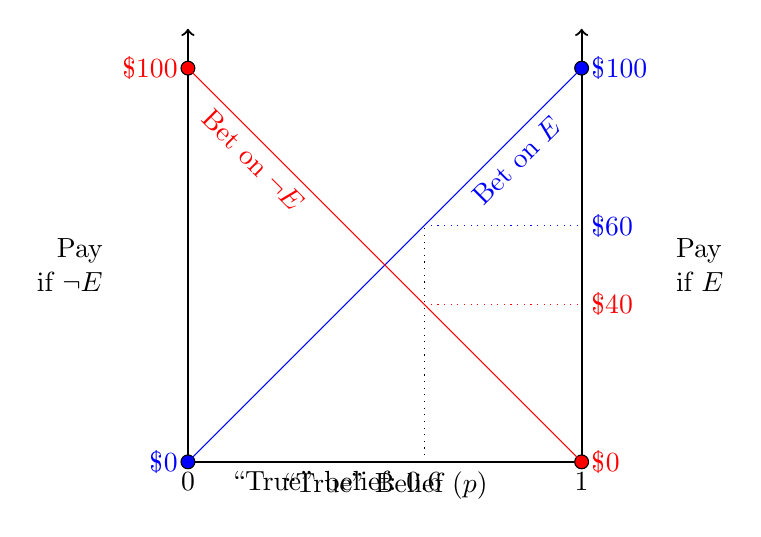
\begin{tikzpicture}[scale=5]
            \draw[thick] (0,0) node[anchor=north]{0} -- (1,0) node[anchor=north]{1};
            \onslide<1>{\node[anchor=north] at (0.5,0) {``True'' Belief ($p$)};}
            \draw[thick,->] (0,0) node[anchor=east]{\color{blue}\$0} -- (0,1) node[anchor=east]{\color{red}\$100} -- (0,1.1);
            \draw[thick,->] (1,0) node[anchor=west]{\color{red}\$0} -- (1,1) node[anchor=west]{\color{blue}\$100} -- (1,1.1);
            \node[align=right] at (-0.3,0.5) {Pay\\if $\neg E$};
            \node[align=left] at (1.3,0.5) {Pay\\if $E$};
            \filldraw[fill=blue] (0,0) circle [radius=0.5pt];
            \filldraw[fill=blue] (1,1) circle [radius=0.5pt];
            \filldraw[fill=red] (0,1) circle [radius=0.5pt];
            \filldraw[fill=red] (1,0) circle [radius=0.5pt];
            \onslide<2->{\draw[blue] (0,0) -- (0.8,0.8) node[anchor=north,rotate=45]{Bet on $E$} -- (1,1);}
            \onslide<2->{\draw[dotted] (0.6,0) node[anchor=north]{\phantom{``}0.6\phantom{''}} -- (0.6,0.6);}
            \onslide<2->{\node[anchor=north] at (0.32,0) {``True'' belief:};}
            \onslide<2->\draw[dotted,blue] (0.6,0.6) -- (1,0.6) node[anchor=west]{\$60};
            \onslide<3->\draw[red] (0,1) -- (0.2,0.8) node[anchor=north,rotate=-45]{Bet on $\neg E$} -- (1,0);
            \onslide<3->\draw[dotted,red] (0.6,0.4) -- (1,0.4) node[anchor=west]{\$40};
        \end{tikzpicture}\br
        How you evaluate these depends on your ``true'' belief\\
        \onslide<2->{Assume (for now) risk-neutral EU}
    \end{center}
\end{frame}

\begin{frame}{Theory: Savage (1971)}
    \begin{center}
        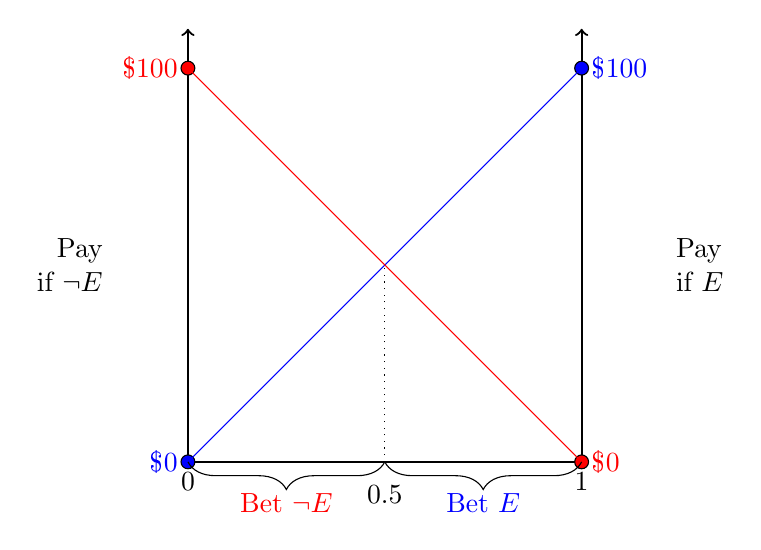
\begin{tikzpicture}[scale=5]
            \draw[thick] (0,0) node[anchor=north]{0} -- (1,0) node[anchor=north]{1};
            \draw[thick,->] (0,0) node[anchor=east]{\color{blue}\$0} -- (0,1) node[anchor=east]{\color{red}\$100} -- (0,1.1);
            \draw[thick,->] (1,0) node[anchor=west]{\color{red}\$0} -- (1,1) node[anchor=west]{\color{blue}\$100} -- (1,1.1);
            \node[align=right] at (-0.3,0.5) {Pay\\if $\neg E$};
            \node[align=left] at (1.3,0.5) {Pay\\if $E$};
            \filldraw[fill=blue] (0,0) circle [radius=0.5pt];
            \filldraw[fill=blue] (1,1) circle [radius=0.5pt];
            \filldraw[fill=red] (0,1) circle [radius=0.5pt];
            \filldraw[fill=red] (1,0) circle [radius=0.5pt];
            \draw[blue] (0,0) -- (1,1);
            \draw[red] (0,1) -- (1,0);
            \draw[dotted] (0.5,0) node[anchor=north,yshift=-5pt]{0.5} -- (0.5,0.5);
            \draw [decorate,decoration={brace,amplitude=10pt,mirror}]
                (0,0) -- (0.5,0) node [red,midway,yshift=-15pt] {Bet $\neg E$};
            \draw [decorate,decoration={brace,amplitude=10pt,mirror}]
                (0.5,0) -- (1,0) node [blue,midway,yshift=-15pt] {Bet $E$};
        \end{tikzpicture}\br
        These two bets separate beliefs into two groups\\
        \onslide<2>{Revelation Principle: ``Is $p\leq0.5$ or is $p\geq0.5$?''}
    \end{center}
\end{frame}

\begin{frame}{Theory: Savage (1971)}
    \begin{center}
        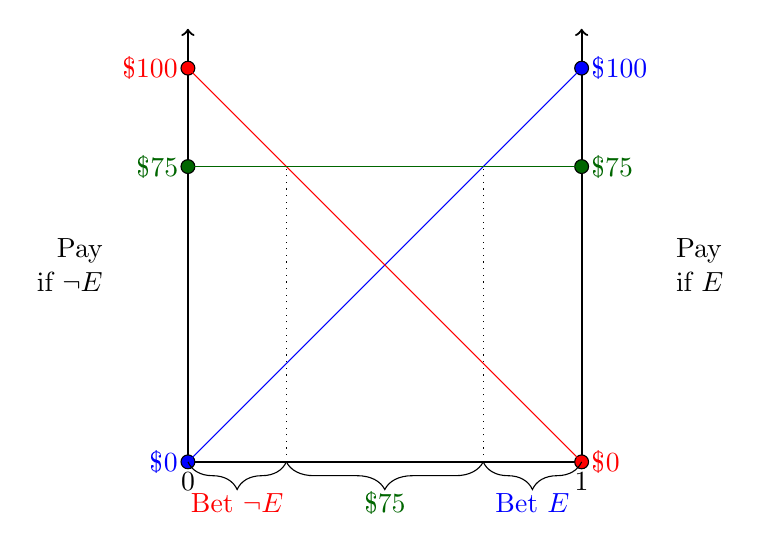
\begin{tikzpicture}[scale=5]
            \draw[thick] (0,0) node[anchor=north]{0} -- (1,0) node[anchor=north]{1};
            \draw[thick,->] (0,0) node[anchor=east]{\color{blue}\$0} -- (0,1) node[anchor=east]{\color{red}\$100} -- (0,1.1);
            \draw[thick,->] (1,0) node[anchor=west]{\color{red}\$0} -- (1,1) node[anchor=west]{\color{blue}\$100} -- (1,1.1);
            \node[align=right] at (-0.3,0.5) {Pay\\if $\neg E$};
            \node[align=left] at (1.3,0.5) {Pay\\if $E$};
            \filldraw[fill=blue] (0,0) circle [radius=0.5pt];
            \filldraw[fill=blue] (1,1) circle [radius=0.5pt];
            \draw[blue] (0,0) -- (1,1);
            \filldraw[fill=red] (0,1) circle [radius=0.5pt];
            \filldraw[fill=red] (1,0) circle [radius=0.5pt];
            \draw[red] (0,1) -- (1,0);
            \filldraw[fill=black!60!green] (0,0.75) circle [radius=0.5pt];
            \filldraw[fill=black!60!green] (1,0.75) circle [radius=0.5pt];
            \draw[black!60!green] (0,0.75) node[anchor=east]{\$75} -- (1,0.75) node[anchor=west]{\$75};
            \draw[dotted] (0.25,0) -- (0.25,0.75);
            \draw[dotted] (0.75,0) -- (0.75,0.75);
            \draw [decorate,decoration={brace,amplitude=10pt,mirror}]
                (0,0) -- (0.25,0) node [red,midway,yshift=-15pt] {Bet $\neg E$};
            \draw [decorate,decoration={brace,amplitude=10pt,mirror}]
                (0.25,0) -- (0.75,0) node [black!60!green,midway,yshift=-15pt] {\$75};
            \draw [decorate,decoration={brace,amplitude=10pt,mirror}]
                (0.75,0) -- (1,0) node [blue,midway,yshift=-15pt] {Bet $E$};
        \end{tikzpicture}\br
        We can get a finer elicitation by adding a constant bet!\\
        \onslide<2>But what about risk aversion...?
    \end{center}
\end{frame}

\begin{frame}{Theory: Savage (1971)}
    \begin{center}
        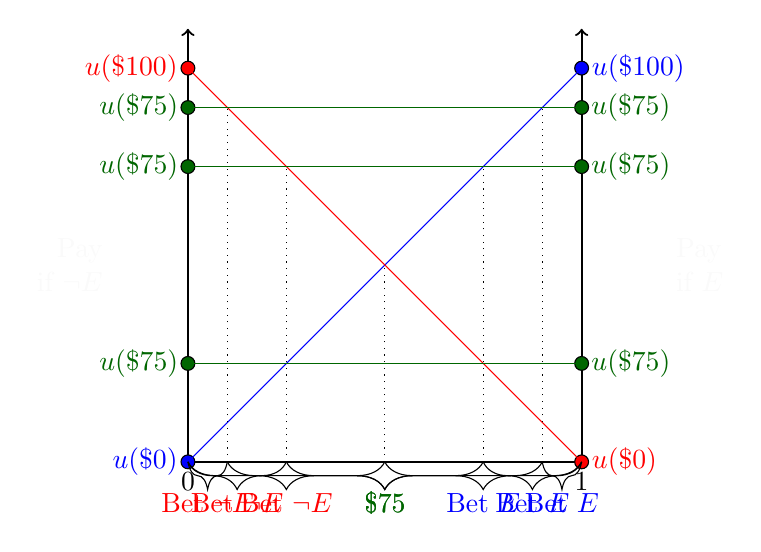
\begin{tikzpicture}[scale=5]
            \node[align=right,color=black!2] at (-0.3,0.5) {Pay\\if $\neg E$};
            \node[align=left,color=black!2] at (1.3,0.5) {Pay\\if $E$};
            \draw[thick] (0,0) node[anchor=north]{0} -- (1,0) node[anchor=north]{1};
            \draw[thick,->] (0,0) node[anchor=east]{\color{blue}$u(\$0)$} -- (0,1) node[anchor=east]{\color{red}$u(\$100)$} -- (0,1.1);
            \draw[thick,->] (1,0) node[anchor=west]{\color{red}$u(\$0)$} -- (1,1) node[anchor=west]{\color{blue}$u(\$100)$} -- (1,1.1);
            \filldraw[fill=blue] (0,0) circle [radius=0.5pt];
            \filldraw[fill=blue] (1,1) circle [radius=0.5pt];
            \draw[blue] (0,0) -- (1,1);
            \filldraw[fill=red] (0,1) circle [radius=0.5pt];
            \filldraw[fill=red] (1,0) circle [radius=0.5pt];
            \draw[red] (0,1) -- (1,0);
            \onslide<1> \filldraw[fill=black!60!green] (0,0.75) circle [radius=0.5pt];
            \onslide<1> \filldraw[fill=black!60!green] (1,0.75) circle [radius=0.5pt];
            \onslide<1> \draw[black!60!green] (0,0.75) node[anchor=east]{$u(\$75)$} -- (1,0.75) node[anchor=west]{$u(\$75)$};
            \onslide<1>\draw[dotted] (0.25,0) -- (0.25,0.75);
            \onslide<1>\draw[dotted] (0.75,0) -- (0.75,0.75);
            \onslide<1> \draw [decorate,decoration={brace,amplitude=10pt,mirror}] (0,0) -- (0.25,0) node [red,midway,yshift=-15pt] {Bet $\neg E$};
            \onslide<1> \draw [decorate,decoration={brace,amplitude=10pt,mirror}] (0.25,0) -- (0.75,0) node [black!60!green,midway,yshift=-15pt] {\$75};
            \onslide<1> \draw [decorate,decoration={brace,amplitude=10pt,mirror}] (0.75,0) -- (1,0) node [blue,midway,yshift=-15pt] {Bet $E$};
            \onslide<2> \filldraw[fill=black!60!green] (0,0.90) circle [radius=0.5pt];
            \onslide<2> \filldraw[fill=black!60!green] (1,0.90) circle [radius=0.5pt];
            \onslide<2> \draw[black!60!green] (0,0.90) node[anchor=east]{$u(\$75)$} -- (1,0.90) node[anchor=west]{$u(\$75)$};
            \onslide<2>\draw[dotted] (0.10,0) -- (0.10,0.90);
            \onslide<2>\draw[dotted] (0.90,0) -- (0.90,0.90);
            \onslide<2> \draw [decorate,decoration={brace,amplitude=10pt,mirror}]
                (0,0) -- (0.10,0) node [red,midway,yshift=-15pt] {Bet $\neg E$};
            \onslide<2> \draw [decorate,decoration={brace,amplitude=10pt,mirror}]
                (0.10,0) -- (0.90,0) node [black!60!green,midway,yshift=-15pt] {\$75};
            \onslide<2> \draw [decorate,decoration={brace,amplitude=10pt,mirror}]
                (0.90,0) -- (1,0) node [blue,midway,yshift=-15pt] {Bet $E$};
            \onslide<3> \filldraw[fill=black!60!green] (0,0.25) circle [radius=0.5pt];
            \onslide<3> \filldraw[fill=black!60!green] (1,0.25) circle [radius=0.5pt];
            \onslide<3> \draw[black!60!green] (0,0.25) node[anchor=east]{$u(\$75)$} -- (1,0.25) node[anchor=west]{$u(\$75)$};
            \onslide<3>\draw[dotted] (0.5,0) -- (0.5,0.5);
            \onslide<3> \draw [decorate,decoration={brace,amplitude=10pt,mirror}] (0,0) -- (0.5,0) node [red,midway,yshift=-15pt] {Bet $\neg E$};
            \onslide<3> \draw [decorate,decoration={brace,amplitude=10pt,mirror}] (0.5,0) -- (1,0) node [blue,midway,yshift=-15pt] {Bet $E$};
        \end{tikzpicture}\br
        \only<1>{Risk neutral}
        \only<2>{Risk averse}
        \only<3>{Risk seeking}\\
        \onslide<3>{Risk preferences $\Rightarrow$ lack of identification};
    \end{center}
\end{frame}

\begin{frame}{Theory: Savage (1971)}
    \begin{center}
        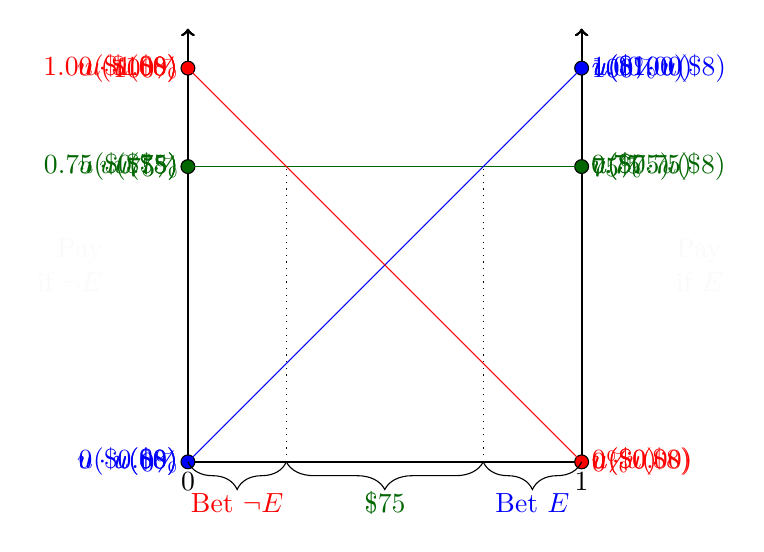
\begin{tikzpicture}[scale=5]
            \node[align=right,color=black!2] at (-0.3,0.5) {Pay\\if $\neg E$};
            \node[align=left,color=black!2] at (1.3,0.5) {Pay\\if $E$};
            \draw[thick] (0,0) node[anchor=north]{0} -- (1,0) node[anchor=north]{1};
            \onslide<1>{\draw[thick,->] (0,0) node[anchor=east]{\color{blue}$u(\$0)$} -- (0,1) node[anchor=east]{\color{red}$u(\$100)$} -- (0,1.1);}
            \onslide<1>{\draw[thick,->] (1,0) node[anchor=west]{\color{red}$u(\$0)$} -- (1,1) node[anchor=west]{\color{blue}$u(\$100)$} -- (1,1.1);}
            \onslide<2>{\draw[thick,->] (0,0) node[anchor=east]{\color{blue}$u(\$0.00)$} -- (0,1) node[anchor=east]{\color{red}$u(\$1.00)$} -- (0,1.1);}
            \onslide<2>{\draw[thick,->] (1,0) node[anchor=west]{\color{red}$u(\$0.00)$} -- (1,1) node[anchor=west]{\color{blue}$u(\$1.00)$} -- (1,1.1);}
            \onslide<3>{\draw[thick,->] (0,0) node[anchor=east]{\color{blue}$0\cdot u(\$8)$} -- (0,1) node[anchor=east]{\color{red}$1.00\cdot u(\$8)$} -- (0,1.1);}
            \onslide<3>{\draw[thick,->] (1,0) node[anchor=west]{\color{red}$0\cdot u(\$8)$} -- (1,1) node[anchor=west]{\color{blue}$1.00\cdot u(\$8)$} -- (1,1.1);}
            \onslide<4->{\draw[thick,->] (0,0) node[anchor=east]{\color{blue}0\%} -- (0,1) node[anchor=east]{\color{red}100\%} -- (0,1.1);}
            \onslide<4->{\draw[thick,->] (1,0) node[anchor=west]{\color{red}0\%} -- (1,1) node[anchor=west]{\color{blue}100\%} -- (1,1.1);}
            \filldraw[fill=black!60!green] (0,0.75) circle [radius=0.5pt];
            \filldraw[fill=black!60!green] (1,0.75) circle [radius=0.5pt];
            \onslide<1>{\draw[black!60!green] (0,0.75) node[anchor=east]{$u(\$75)$} -- (1,0.75) node[anchor=west]{$u(\$75)$};}
            \onslide<2>{\draw[black!60!green] (0,0.75) node[anchor=east]{$u(\$0.75)$} -- (1,0.75) node[anchor=west]{$u(\$0.75)$};}
            \onslide<3>{\draw[black!60!green] (0,0.75) node[anchor=east]{$0.75\cdot u(\$8)$} -- (1,0.75) node[anchor=west]{$0.75\cdot u(\$8)$};}
            \onslide<4->{\draw[black!60!green] (0,0.75) node[anchor=east]{75\%} -- (1,0.75) node[anchor=west]{75\%};}
            \filldraw[fill=blue] (0,0) circle [radius=0.5pt];
            \filldraw[fill=blue] (1,1) circle [radius=0.5pt];
            \draw[blue] (0,0) -- (1,1);
            \filldraw[fill=red] (0,1) circle [radius=0.5pt];
            \filldraw[fill=red] (1,0) circle [radius=0.5pt];
            \draw[red] (0,1) -- (1,0);
            \draw[dotted] (0.25,0) -- (0.25,0.75);
            \draw[dotted] (0.75,0) -- (0.75,0.75);
            \draw [decorate,decoration={brace,amplitude=10pt,mirror}] (0,0) -- (0.25,0) node [red,midway,yshift=-15pt] {Bet $\neg E$};
            \draw [decorate,decoration={brace,amplitude=10pt,mirror}] (0.25,0) -- (0.75,0) node [black!60!green,midway,yshift=-15pt] {\$75};
            \draw [decorate,decoration={brace,amplitude=10pt,mirror}] (0.75,0) -- (1,0) node [blue,midway,yshift=-15pt] {Bet $E$};
        \end{tikzpicture}\br
        \only<1>{Savage (1971) offers 2 solutions...}
        \only<2>{Solution \#1: make payments small (\$1.00)}
        \only<3>{Solution \#2: pay in probabilities}
        \only<4>{``Binarized'' payments (Hossain \& Okui 2013)}
        \only<5>{Solution \#3: estimate risk prefs \& back out $p$}\\
        \only<3>{Payment = \% chance of winning \$8 (\textit{e.g.})}
        \only<4>{Savage (1971) $\rightarrow$ C. Smith (1961) $\rightarrow$ Savage (1954)}
        \only<5>{Offerman et al. (2009), Andersen et al. (2014), etc.}
    \end{center}
\end{frame}

\begin{frame}{Theory: Savage (1971)}
    \begin{center}
        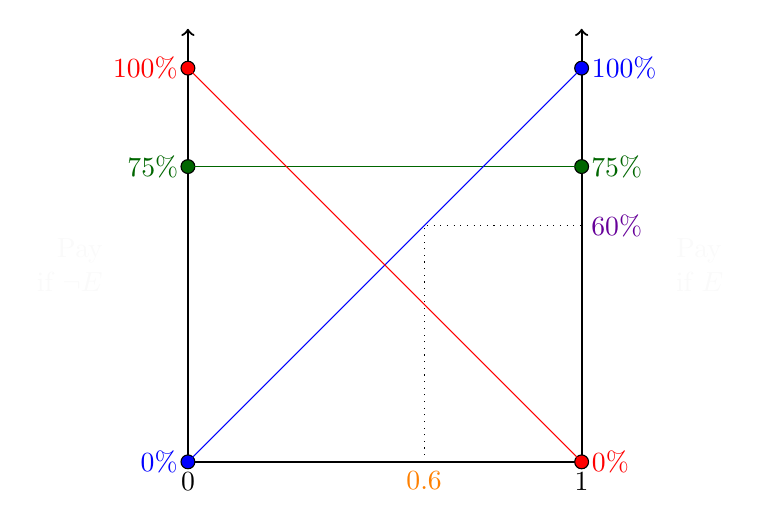
\begin{tikzpicture}[scale=5]
            \node[align=right,color=black!2] at (-0.3,0.5) {Pay\\if $\neg E$};
            \node[align=left,color=black!2] at (1.3,0.5) {Pay\\if $E$};
            \draw[thick] (0,0) node[anchor=north]{0} -- (1,0) node[anchor=north]{1};
            \draw[thick,->] (0,0) node[anchor=east]{\color{blue}0\%} -- (0,1) node[anchor=east]{\color{red}100\%} -- (0,1.1);
            \draw[thick,->] (1,0) node[anchor=west]{\color{red}0\%} -- (1,1) node[anchor=west]{\color{blue}100\%} -- (1,1.1);
            \filldraw[fill=black!60!green] (0,0.75) circle [radius=0.5pt];
            \filldraw[fill=black!60!green] (1,0.75) circle [radius=0.5pt];
            \draw[black!60!green] (0,0.75) node[anchor=east]{75\%} -- (1,0.75) node[anchor=west]{75\%};
            \filldraw[fill=blue] (0,0) circle [radius=0.5pt];
            \filldraw[fill=blue] (1,1) circle [radius=0.5pt];
            \draw[blue] (0,0) -- (1,1);
            \filldraw[fill=red] (0,1) circle [radius=0.5pt];
            \filldraw[fill=red] (1,0) circle [radius=0.5pt];
            \draw[red] (0,1) -- (1,0);
            \draw[dotted] (0.6,0) node[anchor=north]{\color{orange}$0.6$} -- (0.6,0.6) -- (1,0.6) node[anchor=west]{{\color{blue!60!red}60\%}};
        \end{tikzpicture}\br
        \only<1-2>{Still assuming linear preferences: $({\color{orange}0.6}\times{\color{blue}100\%})+({\color{orange}0.4}\times{\color{blue}0\%})={\color{blue!60!red}60\%}$}
        \only<3->{``{\color{orange}Subjective}-{\color{blue}Objective} Reduction''}\\
        \only<1>{{\color{black!2}Booooo}}
        \only<2>{``{\color{orange}Subjective}-{\color{blue}Objective} Reduction'' (aka Binary Reduction)}
        \only<3>{Experimental evidence is pretty negative (Selten et al. 1999, \textit{e.g.})}
        \only<4>{...except in the case of scoring rules (Hossain \& Okui 2013, \textit{e.g.})}
    \end{center}
\end{frame}

\begin{frame}{Theory: Savage (1971)}
    \begin{center}
        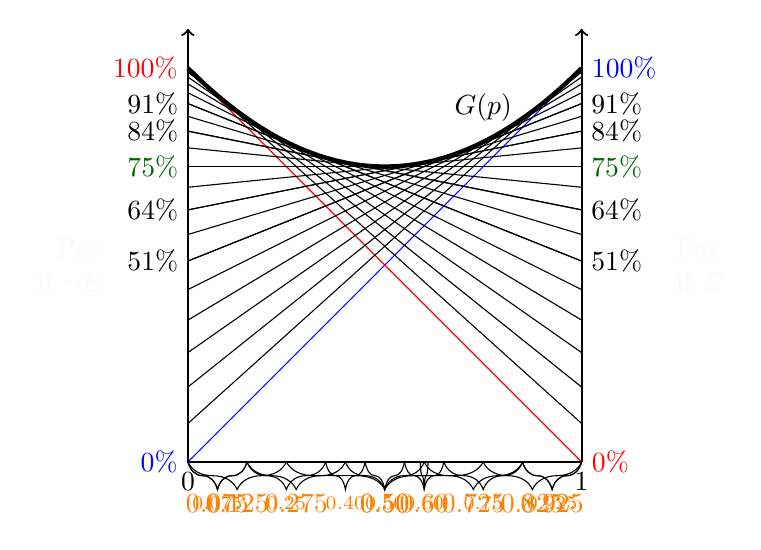
\begin{tikzpicture}[scale=5]
            \node[align=right,color=black!2] at (-0.3,0.5) {Pay\\if $\neg E$};
            \node[align=left,color=black!2] at (1.3,0.5) {Pay\\if $E$};
            \draw[thick] (0,0) node[anchor=north]{0} -- (1,0) node[anchor=north]{1};
            \draw[thick,->] (0,0) node[anchor=east]{\color{blue}0\%} -- (0,1) node[anchor=east]{\color{red}100\%} -- (0,1.1);
            \draw[thick,->] (1,0) node[anchor=west]{\color{red}0\%} -- (1,1) node[anchor=west]{\color{blue}100\%} -- (1,1.1);
            %\filldraw[fill=black!60!green] (0,0.75) circle [radius=0.5pt];
            %\filldraw[fill=black!60!green] (1,0.75) circle [radius=0.5pt];
            \draw[black!60!green] (0,0.75) node[anchor=east]{75\%} -- (1,0.75) node[anchor=west]{75\%};
            %\filldraw[fill=blue] (0,0) circle [radius=0.5pt];
            %\filldraw[fill=blue] (1,1) circle [radius=0.5pt];
            \draw[blue] (0,0) -- (1,1);
            %\filldraw[fill=red] (0,1) circle [radius=0.5pt];
            %\filldraw[fill=red] (1,0) circle [radius=0.5pt];
            \draw[red] (0,1) -- (1,0);
            \foreach \q/\r/\m in {0/.25/125,.25/.75/50,.75/1/825} {
                \onslide<1>{\draw [decorate,decoration={brace,amplitude=10pt,mirror}] (\q,0) -- (\r,0) node [orange,midway,yshift=-15pt] {0.\pgfmathprintnumber{\m}};}
            }
            \foreach \x in {30,70} {
                \pgfmathsetmacro\qsrl{1 - (\x/100)*(\x/100)};
                \pgfmathsetmacro\qsrr{1-(1-\x/100)*(1-\x/100)};
                \pgfmathsetmacro\qsrlo{100*(1 - (\x/100)*(\x/100))};
                \pgfmathsetmacro\qsrro{100*(1-(1-\x/100)*(1-\x/100))};
                \onslide<2->{\draw (0,\qsrl) node[anchor=east]{\pgfmathprintnumber{\qsrlo}\%} -- (1,\qsrr) node[anchor=west]{\pgfmathprintnumber{\qsrro}\%};}
            }
            \foreach \q/\r/\m in {0/.15/075,.15/.4/275,.4/.6/50,.6/.85/725,.85/1/925} {
                \onslide<2>{\draw [decorate,decoration={brace,amplitude=10pt,mirror}] (\q,0) -- (\r,0) node [orange,midway,yshift=-15pt] {0.\m};}
            }
            \foreach \x in {40,60} {
                \pgfmathsetmacro\qsrl{1 - (\x/100)*(\x/100)};
                \pgfmathsetmacro\qsrr{1-(1-\x/100)*(1-\x/100)};
                \pgfmathsetmacro\qsrlo{100*(1 - (\x/100)*(\x/100))};
                \pgfmathsetmacro\qsrro{100*(1-(1-\x/100)*(1-\x/100))};
                \onslide<3->{\draw (0,\qsrl) node[anchor=east]{\pgfmathprintnumber{\qsrlo}\%} -- (1,\qsrr) node[anchor=west]{\pgfmathprintnumber{\qsrro}\%};}
            }
            \foreach \q/\r/\m in {0/.15/075,.15/.35/25,.35/.45/40,.45/.55/50,.55/.65/60,.65/.85/75,.85/1/925} {
                \onslide<3>{\draw [decorate,decoration={brace,amplitude=10pt,mirror}] (\q,0) -- (\r,0) node[orange,midway,yshift=-15pt] {\scriptsize 0.\m};}
            }
            \foreach \x in {5,10,...,95} {
                \pgfmathsetmacro\qsrl{1 - (\x/100)*(\x/100)};
                \pgfmathsetmacro\qsrr{1-(1-\x/100)*(1-\x/100)};
                \onslide<4->{\draw (0,\qsrl) -- (1,\qsrr);}
            }
            \onslide<4->{\draw [decorate,decoration={brace,amplitude=10pt,mirror}] (0.59,0) -- (0.61,0) node[orange,midway,yshift=-15pt] {0.60};}
            \onslide<5>{\draw[domain=0:1, smooth, variable=\y, style={ultra thick}]  plot ({\y}, {(1/2)*(\y*\y+(1-\y)*(1-\y))+(1/2)});}
            \onslide<5>{\node at (0.75,0.9) {$G(p)$};}
        \end{tikzpicture}\br
        \only<1-4>{Now, let's add even more options to the menu...}
        \only<5>{Convex upper envelope: $G(p)$}\\
        \only<2>{5 categories}
        \only<3>{7 categories}
        \only<4>{$\uparrow$ \# bets $\rightarrow$ can elicit an exact $p$}
        \only<5>{Each line is a tangent}
    \end{center}
\end{frame}

\begin{frame}{Theory: Savage (1971)}
    \begin{center}
        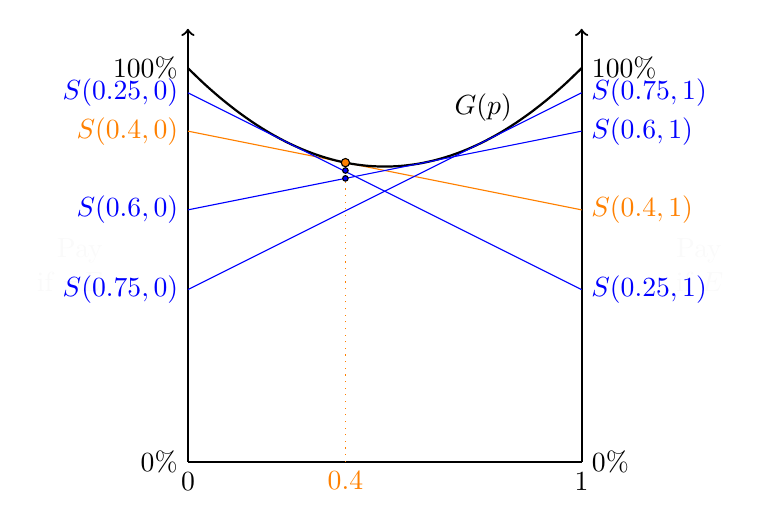
\begin{tikzpicture}[scale=5]
            \node[align=right,color=black!2] at (-0.3,0.5) {Pay\\if $\neg E$};
            \node[align=left,color=black!2] at (1.3,0.5) {Pay\\if $E$};
            \draw[thick] (0,0) node[anchor=north]{0} -- (1,0) node[anchor=north]{1};
            \draw[thick,->] (0,0) node[anchor=east]{0\%} -- (0,1) node[anchor=east]{100\%} -- (0,1.1);
            \draw[thick,->] (1,0) node[anchor=west]{0\%} -- (1,1) node[anchor=west]{100\%} -- (1,1.1);
            \foreach \x in {40} {
                \pgfmathsetmacro\qsrl{1 - (\x/100)*(\x/100)};
                \pgfmathsetmacro\qsrr{1-(1-\x/100)*(1-\x/100)};
                \pgfmathsetmacro\qsrlo{100*(1 - (\x/100)*(\x/100))};
                \pgfmathsetmacro\qsrro{100*(1-(1-\x/100)*(1-\x/100))};
                \pgfmathsetmacro\divhun{\x/100};
                \onslide<1->{\draw[orange] (0,\qsrl) node[anchor=east]{$S(\pgfmathprintnumber[precision=2]{\divhun},0)$} -- (1,\qsrr) node[anchor=west]{$S(\pgfmathprintnumber[precision=2]{\divhun},1)$};}
            }
            \draw[domain=0:1, smooth, variable=\y, style={thick}]  plot ({\y}, {(1/2)*(\y*\y+(1-\y)*(1-\y))+(1/2)});
            \draw[dotted,orange] (0.4,0) node[anchor=north]{0.4} -- (0.4,0.76);
            \filldraw[fill=orange] (0.4,0.76) circle [radius=0.3pt];
            \foreach \x in {60} {
                \pgfmathsetmacro\qsrl{1 - (\x/100)*(\x/100)};
                \pgfmathsetmacro\qsrr{1-(1-\x/100)*(1-\x/100)};
                \pgfmathsetmacro\qsrlo{100*(1 - (\x/100)*(\x/100))};
                \pgfmathsetmacro\qsrro{100*(1-(1-\x/100)*(1-\x/100))};
                \pgfmathsetmacro\divhun{\x/100};
                \onslide<2->{\draw[blue] (0,\qsrl) node[anchor=east]{$S(\pgfmathprintnumber[precision=2]{\divhun},0)$} -- (1,\qsrr) node[anchor=west]{$S(\pgfmathprintnumber[precision=2]{\divhun},1)$};}
            }
            \onslide<2->{\filldraw[fill=blue] (0.4,0.72) circle [radius=0.2pt];}
            \foreach \x in {25} {
                \pgfmathsetmacro\qsrl{1 - (\x/100)*(\x/100)};
                \pgfmathsetmacro\qsrr{1-(1-\x/100)*(1-\x/100)};
                \pgfmathsetmacro\qsrlo{100*(1 - (\x/100)*(\x/100))};
                \pgfmathsetmacro\qsrro{100*(1-(1-\x/100)*(1-\x/100))};
                \pgfmathsetmacro\divhun{\x/100};
                \onslide<3->{\draw[blue] (0,\qsrl) node[anchor=east]{$S(\pgfmathprintnumber[precision=2]{\divhun},0)$} -- (1,\qsrr) node[anchor=west]{$S(\pgfmathprintnumber[precision=2]{\divhun},1)$};}
            }
            \onslide<3->{\filldraw[fill=blue] (0.4,0.74) circle [radius=0.2pt];}
            \foreach \x in {75} {
                \pgfmathsetmacro\qsrl{1 - (\x/100)*(\x/100)};
                \pgfmathsetmacro\qsrr{1-(1-\x/100)*(1-\x/100)};
                \pgfmathsetmacro\qsrlo{100*(1 - (\x/100)*(\x/100))};
                \pgfmathsetmacro\qsrro{100*(1-(1-\x/100)*(1-\x/100))};
                \pgfmathsetmacro\divhun{\x/100};
                \onslide<7->{\draw[blue] (0,\qsrl) node[anchor=east]{$S(\pgfmathprintnumber[precision=2]{\divhun},0)$} -- (1,\qsrr) node[anchor=west]{$S(\pgfmathprintnumber[precision=2]{\divhun},1)$};}
            }
            \onslide<1->{\node at (0.75,0.9) {$G(p)$};}
        \end{tikzpicture}\br
        \only<1-3>{Scoring Rule: Announce $q$.}
        \only<4>{\color{black!2}Booooo}
        \only<5>{\textbf{Theorem (Savage/Schervish):} A mechanism $S(p,X_E)$ is proper iff}
        \only<6>{\textit{Any} convex $G(p)$ will work.}
        \only<7>{$S(q,0)=(1-(0-q)^2)$}
        \\
        \only<1>{If $\neg E$, pay {\color{blue}$S(q,0)$}. \hspace{2cm} If $E$, pay {\color{blue}$S(q,1)$}.}
        \only<2-3>{Announcing ${\color{blue}q}\neq {\color{orange}p}$ gives a lower ${\color{orange}(1-p)}\cdot{\color{blue}S(q,0)}+{\color{orange}p}\cdot{\color{blue}S(q,1)}$}
        \only<4>{$G(p) = $ ${\color{orange}(1-p)\cdot S(p,0) + p\cdot S(p,1)}$}
        \only<5>{the resulting lines are the tangents of a convex function $G(p)$.}
        \only<6>{Binarized \uline{Quadratic scoring rule} (BSR), logarithmic, spherical...}
        \only<7>{$S(q,1)=(1-(1-q)^2)$}
    \end{center}
\end{frame}

\begin{frame}{Issues With the Quadratic Scoring Rule}
    \begin{center}
        \begin{tikzpicture}[scale=5]
            \node[align=right,color=black!2] at (-0.3,0.5) {Pay\\if $\neg E$};
            \node[align=left,color=black!2] at (1.3,0.5) {Pay\\if $E$};
            \draw[thick] (0,0) node[anchor=north]{} -- (1,0) node[anchor=north]{};
            \draw[thick,->] (0,0) node[anchor=east]{0\%} -- (0,1) -- (0,1.1);
            \draw[thick,->] (1,0) node[anchor=west]{0\%} -- (1,1) -- (1,1.1);
            \foreach \x in {60} {
                \pgfmathsetmacro\qsrl{1 - (\x/100)*(\x/100)}
                \pgfmathsetmacro\qsrr{1-(1-\x/100)*(1-\x/100)}
                \pgfmathsetmacro\qsrlo{100*(1 - (\x/100)*(\x/100))}
                \pgfmathsetmacro\qsrro{100*(1-(1-\x/100)*(1-\x/100))}
                \only<1>{\draw[blue] (0,\qsrl) node[anchor=east]{\pgfmathprintnumber{\qsrlo}\%} -- (1,\qsrr) node[anchor=west]{\pgfmathprintnumber{\qsrro}\%}};
            }
            \only<1>{\draw[dotted] (0.4,0) node[anchor=north]{\color{orange}0.40} -- (0.4,0.72) -- (1,0.72) node[anchor=west] {\color{red!50!blue}72\%}};
            \foreach \x in {5,25} {
                \pgfmathsetmacro\qsrl{1 - (\x/100)*(\x/100)}
                \pgfmathsetmacro\qsrr{1-(1-\x/100)*(1-\x/100)}
                \pgfmathsetmacro\qsrlo{100*(1 - (\x/100)*(\x/100))}
                \pgfmathsetmacro\qsrro{100*(1-(1-\x/100)*(1-\x/100))}
                \pgfmathsetmacro\bigg{(1/2)*((\x/100)*(\x/100) + (1-\x/100)*(1-\x/100))+(1/2)}
                \pgfmathsetmacro\divhun{\x/100}
                \only<2->{\draw (0,\qsrl) node[anchor=east]{\pgfmathprintnumber{\qsrlo}\%} -- (1,\qsrr) node[anchor=west]{\pgfmathprintnumber{\qsrro}\%}};
                \only<2->{\draw[dotted,orange] (\divhun,0) node[anchor=north]{\footnotesize \pgfmathprintnumber[fixed]{\divhun}} -- (\divhun,\bigg)};
            }
            \foreach \x in {10,15,20} {
                \pgfmathsetmacro\qsrl{1 - (\x/100)*(\x/100)}
                \pgfmathsetmacro\qsrr{1-(1-\x/100)*(1-\x/100)}
                \pgfmathsetmacro\qsrlo{100*(1 - (\x/100)*(\x/100))}
                \pgfmathsetmacro\qsrro{100*(1-(1-\x/100)*(1-\x/100))}
                \only<2->{\draw (0,\qsrl) node[anchor=east]{} -- (1,\qsrr) node[anchor=west]{\pgfmathprintnumber{\qsrro}\%}};
            }
            \draw[domain=0:1, smooth, variable=\y, style={ultra thick}]  plot ({\y}, {(1/2)*(\y*\y+(1-\y)*(1-\y))+(1/2)});
            \node at (0.75,0.9) {$G(p)$};
        \end{tikzpicture}\br
        \only<1>{Concern \#1: IC calculation requires {\color{orange}S}-{\color{blue}O} Reduction}
        \only<2>{Concern \#2: $S'(p,0)$ vs $S'(p,1)$}
        \only<3>{But see FOC: $pS'(p,1)+(1-p)S'(p,0)=0$}
        \only<4>{Relative slopes are pinned down by IC!}\\
        \only<1>{$({\color{orange}0.4}\cdot{\color{blue}84\%})+({\color{orange}0.6}\cdot{\color{blue}64\%})=\color{red!50!blue}72\%$}
        \only<2>{See Danz, Wilson \& Vesterlund (2020), \textit{e.g.}}
        \only<3>{$\Rightarrow p/(1-p) = -S'(p,0)/S'(p,1)$}
        \only<4>{\textbf{Corollary:} For \textit{any} IC scoring rule, $S'(p,0)/S'(p,1)=-p/(1-p)$.}
    \end{center}
\end{frame}

\begin{frame}{An Alternative Visualization}
\begin{center}
        \usetikzlibrary{math}
        \begin{tikzpicture}[scale=4]
          \draw[->,line width=1.5](0,0)--(1.2,0) node [below right] {$s_1=Pr(\$8|E)$};
          \draw[->,line width=1.5](0,0)--(0,1.2) node [left] {$Pr(\$8|\neg E)=s_0$};
          \node[below] at (1,0) {$1$};
          \node[left] at (0,1) {$1$};
          \draw[dotted](0,0)--(1,1) node[above right] {$45^\circ$};
          \tikzmath{\ua = 12; \ub = 1; \us = 1.6131730308;
          \ulabx = 0.51;
          \ulaby = (\ua/\ub)^(1/(\us-1)) * (1-\ulabx^((\us-1)/\us))^(\us/(\us-1));
          \rlabx = 0.45; \rlaby = 1.5-1.5*0.45;
          \xa = 0.6; \xdel = 0.1; \xb = \xa + \xdel; \ya = 1.9-1.5*\xa; \yb = \ya + 1.5*\xdel;}
          \draw [line width=0.8,domain=0.504:0.95,samples=40] plot ({\x}, {(\ua/\ub)^(1/(\us-1)) * (1-\x^((\us-1)/\us))^(\us/(\us-1))  });
          \node[right] at (\ulabx,\ulaby) {$u(\cdot)$};
          \draw [line width=0.8,domain=1:0.3,dashed] plot (\x,{1.5-1.5*\x});
          \node[left] at (\rlabx,\rlaby) {$R(\cdot|0.6)$};
          \filldraw[black] (0.6,0.6) circle (0.5pt) node[right]{$(0.6,0.6)$};
          \filldraw[black] (1,0) circle (0.5pt) node[above right]{$(1,0)$};
        \end{tikzpicture}\br
\end{center}
 ``Have a belief of 0.6'': $u(1,0)=u(0.6,0.6)$\\
Define $R(s_1,s_0|p)=p\cdot s_1 + (1-p)\cdot s_0$. Linear level curves.\\
\textbf{S-O Reduction:} Have belief $p$ and $u(s_1,s_0)= R(s_1,s_0|p)$
\end{frame}


\begin{frame}{The BQSR}
\begin{center}
        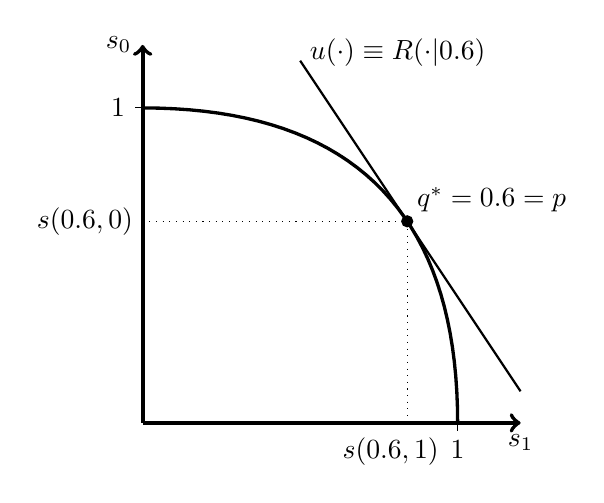
\begin{tikzpicture}[scale=4]
          \draw[->,line width=1.5](0,0)--(1.2,0) node [below] {$s_1$};
          \draw[-,thin] (1,0)--(1,-0.025) node[below] {$1$};
          \draw[-,thin] (0,1)--(-0.025,1) node[left] {$1$};
          \draw[->,line width=1.5](0,0)--(0,1.2) node [left] {$s_0$};
          %\draw[domain=0:1,smooth,line width=1.2] plot (\x,{1-(1-(1-\x)^(1/2))^2});
          \draw [line width=1.2,domain=0:1,samples=40] plot ({1-(1-\x)^2}, {1-(0-\x)^2});
          \filldraw[black] (0.84,0.64) circle (0.5pt) node[above right] {$q^*=0.6=p$};
          \draw[-,dotted] (0,0.64) node[left] {$s(0.6,0)$} -- (0.84,0.64) -- (0.84,0) node[below,label={[xshift=-6pt, yshift=-19pt]{$s(0.6,1)$}}] {};
          %\draw[->,dashed,line width=0.5] (0,0)--(0.84,0.64) node[midway,above left] {};
          %\draw[-,dotted] (0,0.4) node[left] {$0.4$} -- (0.6,0.4) -- (0.6,0) node[below] {$p=0.6$};
          \draw [line width=0.8,domain=0.5:1.2] plot (\x,{1.9-(1.5)*\x});
          \node[above right] at (0.5,1.1) {$u(\cdot)\equiv R(\cdot|0.6)$};
        \end{tikzpicture}
\end{center}
        \only<1>{Binarized Quadratic Scoring Rule forms quarter-circle as you vary $q$\\
        Maximizing point given $u(\cdot)\equiv R(\cdot|0.6)$ is $q^*=0.6$}
        \only<2>{\textit{Any} strictly concave shape corresponds\\
        to some proper scoring rule}
\end{frame}

\begin{frame}{Necessity of S-O Reduction}
\begin{center}
    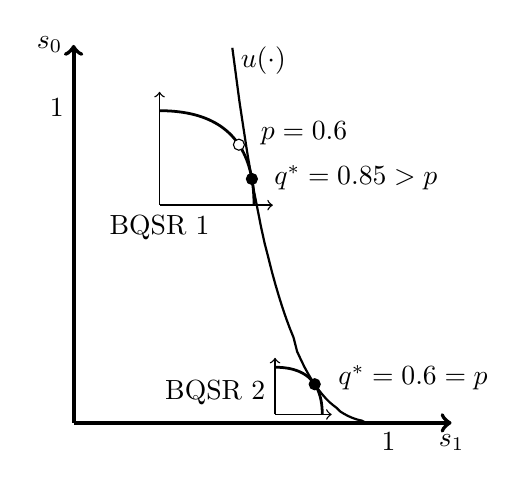
\begin{tikzpicture}[scale=4]
          \draw[->,line width=1.5](0,0)--(1.2,0) node [below] {$s_1$};
          \node[below] at (1,0) {$1$};
          \node[left] at (0,1) {$1$};
          \draw[->,line width=1.5](0,0)--(0,1.2) node [left] {$s_0$};
          %\draw[domain=0:1,smooth,line width=1.2] plot (\x,{1-(1-(1-\x)^(1/2))^2});
          %\tikzmath{\ua = 12; \ub = 1; \us = 1.6131730308; \ulabx = 0.51; \ulaby = (\ua/\ub)^(1/(\us-1)) * (1-\ulabx^((\us-1)/\us))^(\us/(\us-1));}
          \draw [line width=0.8,domain=0.504:0.95,samples=40] plot ({\x}, {(12)^(1/(1.6131730308-1)) * (1-\x^((1.6131730308-1)/1.6131730308))^(1.6131730308/(1.6131730308-1))  });
          \node[right] at (0.5,1.15) {$u(\cdot)$};
          
          \draw[->,line width=0.5] (0.6396,0.02671) node[above left] {BQSR 2} -- (0.8196,0.02671);
          \draw[->,line width=0.5] (0.6396,0.02671) -- (0.6396,0.20671);
          \draw[line width=1.0,domain=0:1,samples=40] plot ({0.6396 + 0.15*(1-(1-\x)^2)}, {0.02671 + 0.15*(1-(0-\x)^2)});
          \filldraw[black] (0.76560335,0.12271) circle (0.5pt) node[right,label={[xshift=32pt, yshift=-9pt]{$q^*=0.6=p$}}] {};
          \draw[->,line width=0.5] (0.2729,0.69121) node[below] {BQSR 1} -- (0.6329,0.69121);
          \draw[->,line width=0.5] (0.2729,0.69121) -- (0.2729,1.05121);
          \draw[line width=1.0,domain=0:1,samples=40] plot ({0.2729 + 0.3*(1-(1-\x)^2)}, {0.69121 + 0.3*(1-(0-\x)^2)});
          \filldraw[black] (0.56614854,0.77446) circle (0.5pt) node[right,label={[xshift=34pt, yshift=-11pt]{$q^*=0.85>p$}}] {};
          \draw[draw=black,fill=white] (0.5249,0.88321) circle (0.5pt) node[right,label={[xshift=20pt, yshift=-7pt]{$p=0.6$}}] {};
        \end{tikzpicture}
\end{center}
\textbf{Know:} If S-O Reduction then every scaled BQSR is IC\\
If $u(\cdot)\not\equiv R(\cdot|p)$ then $\exists$ scaled BQSR that's not IC.\\
\textbf{Proposition:} If every scaled BQSR is IC then \only<1>{$u(\dot)\equiv R(\cdot|p)$}\only<2>{\textit{S-O Reduction}}
\end{frame}

\begin{frame}{More Than One Event}
\begin{itemize}
    \item Suppose multiple events $E_1, E_2, \ldots, E_m$
    \item Want to elicit $p=(p_1,\ldots,p_m)$
    \item Let $X = i$ iff $\omega\in E_i$
    \item Announcement: $q=(q_1,\ldots,q_m)$
\end{itemize}
Quadratic Scoring Rule (scaled to $[0,1]$):
$$
    S(q,i) = 1 - \frac{m}{m-1}\sum_{j=1}^m (\mathbbm{1}_{\{X=j\}} - q_j)^2
$$
Scaled BQSR:
\begin{align*}
    S(q,i) &= \beta_i - \alpha \sum_{j=1}^m (\mathbbm{1}_{\{X=j\}} - q_j)^2\\
    & 0 < \beta_j \leq 1\ \ \forall j \\
    & 0 < \alpha \leq \frac{m-1}{m} \min_j \beta_j
\end{align*}
\end{frame}

\begin{frame}{Other Scoring Rules}
(These are not necessarily scaled to $[0,1]$)
\begin{enumerate}
    \item Spherical Scoring Rule (Roby 1964)
    $$
        S(q,i) = \frac{q_i^2}{\sqrt{\sum_{j=1}^m q_j^2)}}
    $$
    \item Generalized Spherical Scoring Rule ($\lambda > 1$)
    $$
        S(q,i) = \frac{q_i^\lambda}{(\sum_{j=1}^m q_j^\lambda)^{(\lambda-1)/\lambda}}
    $$
    \item Logarithmic Scoring Rule
    $$
        S(q,i) = \log q_i
    $$
    (goes to $-\infty$, can't be scaled to $[0,1]$)
\end{enumerate}
\end{frame}

\begin{frame}{Comparison of Scoring Rules}
\begin{center}
    \includegraphics[width=4.5in]{LectureSlides/graphics/blf/ScoringRuleGs.png}
\end{center}
\end{frame}


\begin{frame}{(Non-Proper) Linear Scoring Rule}
    \begin{center}
        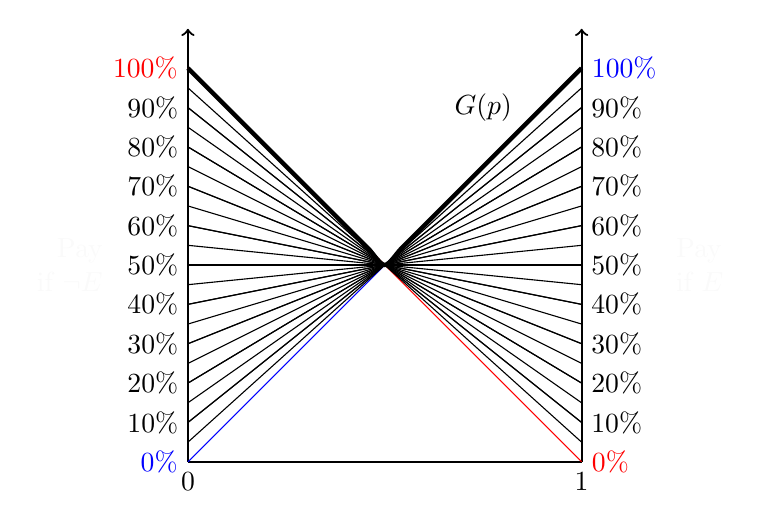
\begin{tikzpicture}[scale=5]
            \node[align=right,color=black!2] at (-0.3,0.5) {Pay\\if $\neg E$};
            \node[align=left,color=black!2] at (1.3,0.5) {Pay\\if $E$};
            \draw[thick] (0,0) node[anchor=north]{0} -- (1,0) node[anchor=north]{1};
            \draw[thick,->] (0,0) node[anchor=east]{\color{blue}0\%} -- (0,1) node[anchor=east]{\color{red}100\%} -- (0,1.1);
            \draw[thick,->] (1,0) node[anchor=west]{\color{red}0\%} -- (1,1) node[anchor=west]{\color{blue}100\%} -- (1,1.1);
            %\filldraw[fill=black!60!green] (0,0.75) circle [radius=0.5pt];
            %\filldraw[fill=black!60!green] (1,0.75) circle [radius=0.5pt];
            %\draw[black!60!green] (0,0.75) node[anchor=east]{75\%} -- (1,0.75) node[anchor=west]{75\%};
            %\filldraw[fill=blue] (0,0) circle [radius=0.5pt];
            %\filldraw[fill=blue] (1,1) circle [radius=0.5pt];
            \draw[blue] (0,0) -- (1,1);
            %\filldraw[fill=red] (0,1) circle [radius=0.5pt];
            %\filldraw[fill=red] (1,0) circle [radius=0.5pt];
            \draw[red] (0,1) -- (1,0);
            %\foreach \q/\r/\m in {0/.25/125,.25/.75/50,.75/1/825} {
            %    \onslide<1>{\draw [decorate,decoration={brace,amplitude=10pt,mirror}] (\q,0) -- (\r,0) node [orange,midway,yshift=-15pt] {0.\pgfmathprintnumber{\m}};}
            %}
            \foreach \x in {20,70} {
                \pgfmathsetmacro\qsrl{1 - (\x/100)};
                \pgfmathsetmacro\qsrr{(\x/100)};
                \pgfmathsetmacro\qsrlo{100*(1 - (\x/100))};
                \pgfmathsetmacro\qsrro{100*(\x/100)};
                \onslide<2->{\draw (0,\qsrl) node[anchor=east]{\pgfmathprintnumber{\qsrlo}\%} -- (1,\qsrr) node[anchor=west]{\pgfmathprintnumber{\qsrro}\%};}
            }
            %\foreach \q/\r/\m in {0/.15/075,.15/.4/275,.4/.6/50,.6/.85/725,.85/1/925} {
            %    \onslide<2>{\draw [decorate,decoration={brace,amplitude=10pt,mirror}] (\q,0) -- (\r,0) node [orange,midway,yshift=-15pt] {0.\m};}
            %}
            \foreach \x in {10,30,40,50,60,80,90} {
                \pgfmathsetmacro\qsrl{1 - (\x/100)};
                \pgfmathsetmacro\qsrr{(\x/100)};
                \pgfmathsetmacro\qsrlo{100*(1 - (\x/100))};
                \pgfmathsetmacro\qsrro{100*(\x/100)};
                \onslide<3->{\draw (0,\qsrl) node[anchor=east]{\pgfmathprintnumber{\qsrlo}\%} -- (1,\qsrr) node[anchor=west]{\pgfmathprintnumber{\qsrro}\%};}
            }
            % \foreach \q/\r/\m in {0/.15/075,.15/.35/25,.35/.45/40,.45/.55/50,.55/.65/60,.65/.85/75,.85/1/925} {
            %     \onslide<3>{\draw [decorate,decoration={brace,amplitude=10pt,mirror}] (\q,0) -- (\r,0) node[orange,midway,yshift=-15pt] {\scriptsize 0.\m};}
            % }
            \foreach \x in {5,10,...,95} {
                \pgfmathsetmacro\qsrl{1 - (\x/100)};
                \pgfmathsetmacro\qsrr{(\x/100)};
                \onslide<4->{\draw (0,\qsrl) -- (1,\qsrr);}
            }
            % \onslide<4->{\draw [decorate,decoration={brace,amplitude=10pt,mirror}] (0.59,0) -- (0.61,0) node[orange,midway,yshift=-15pt] {0.60};}
            \onslide<5>{\draw[domain=0:1, smooth, variable=\y, style={ultra thick}]  plot ({\y}, {max(\y,1-\y)});}
            \onslide<5>{\node at (0.75,0.9) {$G(p)$};}
        \end{tikzpicture}\br
        \only<1-4>{$S(q,0)=1-q$\hspace{1in}$S(q,1)=q$}
        \only<5>{Convex upper envelope: $G(p)$}\\
        \only<1>{Same extremes as QSR}
        \only<2-4>{But now symmetric slopes}
        \only<5>{$q^*=0$ if $p<50$, $q^*=100$  if $p>50$}
    \end{center}
\end{frame}

\begin{frame}{Characterizations of the QSR}
Selten (1998, \textit{ExpEcon} v.1)
\begin{itemize}
    \item \textbf{Symmetry}: $S(q,i)=S(\pi(q),\pi(i))$ for any permutation $\pi$
    \item \textbf{Elongation Invariance:} $S((q_1,\ldots,q_n),i)=S((q_1,\ldots,q_n,0),i)$ (adding a null event)
    \item \textbf{Neutrality:} $G(q|p)=G(p|q)$
    \item \textbf{Properness:} $S$ is proper
\end{itemize}
\br
\textbf{Theorem:} A scoring rule satisfies these 4 axioms iff it is a scaled QSR
\end{frame}

\begin{frame}{Characterizations of the QSR}
\begin{itemize}
    \item Suppose we impose a grid $\mathcal{G}=\{0,\frac{1}{k},\frac{2}{k},\ldots,\frac{k-1}{k},1\}$
    \item Require each $q_i\in \mathcal{G}$
    \item \textbf{Midpoint Property:} Optimal announcement is $q_i^*=\frac{r}{k}$ if and only if $p_i\in [\frac{r}{k}-\frac{1}{2k},\frac{r}{k}+\frac{1}{2k}]$
    \begin{itemize}
        \item Ensures that the announced point is the closest grid point to the true belief.
    \end{itemize}
\end{itemize}
\br
\textbf{Theorem:} The Scaled QSRs are the only proper scoring rules with the midpoint property
    
\end{frame}

\begin{frame}{Characterizations of the QSR}
\begin{itemize}
    \item We want to maximize the incentive not to deviate
    \item Local incentive not to deviate at $q=p$
    $$
        G''(q=p|p) = G''(p)
    $$
    \item BQSR has $G''\equiv 2$
    \item Any binarized rule must have $G'(0)\geq -1$, $G'(1)\leq 1$
    \begin{itemize}
        \item All lines in the graph must have slope in $[-1,1]$
    \end{itemize}
    \item Thus, $\int_0^1 G''(p)dp = G'(1)-G'(0) \leq 2$
    \item Any other scoring rule has $G''(p)<2$ at some $p$
\end{itemize}
\br
\textbf{Theorem:} The (unscaled) BQSR maximizes $\min_p G''(p)$
\br
Related: Schlag, Tremewan \& van der Weele (2015)
\end{frame}

\begin{frame}{A Different Scoring Rule}
    \begin{center}
        \begin{tikzpicture}[scale=5]
            \node[align=right,color=black!2] at (-0.3,0.5) {Pay\\if $\neg E$};
            \node[align=left,color=black!2] at (1.3,0.5) {Pay\\if $E$};
            \draw[thick] (0,0) node[anchor=north]{} -- (1,0) node[anchor=north]{};
            \draw[thick,->] (0,0) node[anchor=east]{} -- (0,1) -- (0,1.1);
            \draw[thick,->] (1,0) node[anchor=west]{0\%} -- (1,1) -- (1,1.1);
            \foreach \x in {0} {
                \pgfmathsetmacro\qsrl{(1 - (\x/100)*(\x/100))*(1/2)}
                \pgfmathsetmacro\qsrr{(1-(1-\x/100)*(1-\x/100))*(1/2) + 1/2}
                \pgfmathsetmacro\qsrlo{50*(1 - (\x/100)*(\x/100))}
                \pgfmathsetmacro\qsrro{50*(1-(1-\x/100)*(1-\x/100)) + 50}
                \only<1->{\draw[black!60!green] (0,\qsrl) node[anchor=east]{\pgfmathprintnumber{\qsrlo}\%} -- (1,\qsrr) node[anchor=west]{\pgfmathprintnumber{\qsrro}\%}};
            }
            \foreach \x in {100} {
                \pgfmathsetmacro\qsrl{(1 - (\x/100)*(\x/100))*(1/2)}
                \pgfmathsetmacro\qsrr{(1-(1-\x/100)*(1-\x/100))*(1/2) + 1/2}
                \pgfmathsetmacro\qsrlo{50*(1 - (\x/100)*(\x/100))}
                \pgfmathsetmacro\qsrro{50*(1-(1-\x/100)*(1-\x/100)) + 50}
                \only<1->{\draw[blue] (0,\qsrl) node[anchor=east]{\pgfmathprintnumber{\qsrlo}\%} -- (1,\qsrr) node[anchor=west]{\pgfmathprintnumber{\qsrro}\%}};
            }
            \foreach \x in {40,60} {
                \pgfmathsetmacro\qsrl{(1 - (\x/100)*(\x/100))*(1/2)}
                \pgfmathsetmacro\qsrr{(1-(1-\x/100)*(1-\x/100))*(1/2) + 1/2}
                \pgfmathsetmacro\qsrlo{50*(1 - (\x/100)*(\x/100))}
                \pgfmathsetmacro\qsrro{50*(1-(1-\x/100)*(1-\x/100)) + 50}
                \only<1->{\draw[] (0,\qsrl) node[anchor=east]{\pgfmathprintnumber{\qsrlo}\%} -- (1,\qsrr) node[anchor=west]{\pgfmathprintnumber{\qsrro}\%}};
            }
            \draw[domain=0:1, smooth, variable=\y, style={ultra thick}]  plot ({\y}, {(1/2)*(1+ \y*\y});
            \node at (0.75,0.9) {$G(p)$};
        \end{tikzpicture}\br
        \only<1>{A new IC scoring rule}
        \only<2>{$S(q,0)=\frac{1}{2}(1-q^2)$}
        \only<3>{$S(q,0)={\color{red}\frac{1}{2}}(1-q^2)$}
        \only<4>{\textbf{Magic Trick:} I'll show \textit{this} scoring rule can be IC}\\
        \only<1>{$G(p) = \frac{1}{2}(1+q^2)$}
        \only<2>{$S(q,1)=\frac{1}{2}(1-(1-q)^2)+\frac{1}{2}$}
        \only<3>{$S(q,1)={\color{red}\frac{1}{2}}(1-(1-q)^2)+{\color{red}\frac{1}{2}}$}
        \only<4>{\emph{without} relying on S-O Reduction}
    \end{center}
\end{frame}

\begin{frame}{Breaking Apart Reduction}
Consider the S-O-Reduced $Pr(\$8)$:
\begin{center}
    \begin{align*}
        & {\color{orange}p}\cdot({\color{blue}\underbrace{\frac{1}{2}(1-(1-q)^2)+\frac{1}{2}}_{S(q,1)}}) + {\color{orange}(1-p)}\cdot{\color{blue}\underbrace{\frac{1}{2}(1-q^2)}_{S(q,0)}}\\
        = & {\color{blue}q}\cdot {\color{orange}p} + {\color{blue}(1-q)}\only<1-2>{\color{blue}\left(\frac{1}{2}q + \frac{1}{2}1\right)}\only<3->{\color{blue!50!green}\left(\frac{1}{2}q + \frac{1}{2}1\right)}
    \end{align*}\br
    \only<1>{\begin{tabular}{c}{\color{black!2}Booo}\\{\color{black!2}Booo}\end{tabular}\br {\color{black!2}Adding a second objective randomizing device}}
    \only<2>{\begin{tabular}{rl}
    {\color{blue}$q$}&: get a \$8 bet on {\color{orange}$E$}\\
    {\color{blue}$(1-q)$}&: get a lottery that pays \$8 w/ prob {\color{blue}$\left(\frac{1}{2}q + \frac{1}{2}1\right)$}
    \end{tabular}\br {\color{black!2}Adding a second objective randomizing device}}
    \only<3->{\begin{tabular}{rl}
    {\color{blue}$q$}&: get a \$8 bet on {\color{orange}$E$}\\
    {\color{blue}$(1-q)$}&: get a lottery that pays \$8 w/ prob {\color{blue!50!green}$\left(\frac{1}{2}q + \frac{1}{2}1\right)$}
    \end{tabular}\br Adding a second objective randomizing device}
\end{center}
\end{frame}

\begin{frame}{Breaking Apart Reduction}
    \begin{center}
        $${\color{blue}q}\cdot {\color{orange}p} + {\color{blue}(1-q)}\color{blue!50!green}\frac{q+1}{2}$$
        Imagine 100 rows. Announce $q\in[0,100]$. Payment:\\
        \begin{align*}
        {\color{blue}q}\left \{\begin{array}{cc}
        \mathrm{\$8\ if\ }E & {\color{black!2}\mathrm{\$8\ w/\ prob\ }q+1\mathrm{\%}}\\
        \mathrm{\$8\ if\ }E & {\color{black!2}\mathrm{\$8 w/ prob 10\%}}\\
        \vdots & \\
        \mathrm{\$8\ if\ }E & {\color{black!2}\mathrm{\$8 w/ prob 10\%}}\\
        \end{array}
        \right\}&={\color{blue}q}\cdot{\color{orange}p\%} \\
        {\color{blue}(1-q)}\left \{\begin{array}{cc}
        {\color{black!2}\mathrm{\$8\ if\ }E} & \mathrm{\$8\ w/\ prob\ }q+1\mathrm{\%}\\
         & \mathrm{\$8\ w/\ prob\ }q+2\mathrm{\%}\\
         & \vdots \\
         & \mathrm{\$8\ w/\ prob\ 99\%}\\
         & \mathrm{\$8\ w/\ prob\ 100\%}\\
        \end{array}
        \right\}&={\color{blue}(1-q)}\cdot{\color{blue!50!green}\underbrace{\left(\frac{1}{2}q+\frac{1}{2}1\right)}_{\text{Avg. prob. from $q$ to $1$}}\%}
        \end{align*}
    \end{center}
\end{frame}

\begin{frame}{Breaking Apart Reduction: Multiple Price List}
    \begin{center}
    \only<1->{\begin{tabular}{|c|ccc|}
        \hline
        {\color{red}\textbf{Row\#}} & {\color{black!2}aaaa}{\color{red}\textbf{Option A}}{\color{black!2}aaaa} & OR & {\color{red}\textbf{Option B}} \\
        \hline
        1 & \hugme{\$8 if $E$} & or & \$8 w/ prob 1\%\\
        \hline
        2 & \hugme{\$8 if $E$} & or & \$8 w/ prob 2\%\\
        \hline
        $\vdots$ & $\vdots$ & $\vdots$ & $\vdots$\\
        \hline
        $q$ & \hugme{\$8 if $E$} & or & \$8 w/ prob $q$\%\\
        \hline
        $q+1$ & \$8 if $E$ & or & \hugme{\$8 w/ prob $q+1$\%}\\
        \hline
        $\vdots$ & $\vdots$ & $\vdots$ & $\vdots$\\
        \hline
        99 & \$8 if $E$ & or & \hugme{\$8 w/ prob 99\%}\\
        \hline
        100 & \$8 if $E$ & or & \hugme{\$8 w/ prob 100\%}\\
        \hline
    \end{tabular}}
    \br
    \only<1>{Equivalently: Choose Option A or Option B}
    \only<2>{``Multiple Price List'' (MPL) version of BDM for probabilities}
    \only<3-4>{One row randomly selected for payment}
    \only<5>{\textbf{Summary:} Took a scoring rule, converted it into an MPL}
    \\
    \only<1>{Choice of $q$ determines your choices}
    \only<2>{Holt \& Smith (2016), others}
    \only<3>{If you lie, you get the less-preferred option on some rows}
    \only<4>{I.C. as long as subject respects statewise dominance}
    \only<5>{Now IC does \emph{not} require S-O Reduction!}
    \end{center}
\end{frame}

% \begin{frame}{The MPL}
%     \begin{center}
%     My belief $q$ is: \begin{tabular}{|c|}
%         \hline
%         \only<1>{{\color{black!2}50}}
%         \only<2>{{\color{blue}56}}
%         \only<3>{{\color{blue}58}}\\
%         \hline
%     \end{tabular}\\
%     \begin{tabular}{|c|ccc|}
%         \hline
%         {\color{red}\textbf{Row\#}} & {\color{black!2}aaaa}{\color{red}\textbf{Option A}}{\color{black!2}aaaa} & OR & {\color{red}\textbf{Option B}} \\
%         \hline
%         $\vdots$ & $\vdots$ & $\vdots$ & $\vdots$\\
%         \hline
%         55 & \only<1>{\$8 if $E$}\only<2-3>{\hugme{\$8 if $E$}} & or & \$8 w/ prob 55\%\\
%         \hline
%         56 & \only<1>{\$8 if $E$}\only<2-3>{\hugme{\$8 if $E$}} & or & \$8 w/ prob 56\%\\
%         \hline
%         57 & \only<1-2>{\$8 if $E$}\only<3>{\hugme{\$8 if $E$}} & or & \only<1,3>{\$8 w/ prob 57\%}\only<2>{\hugme{\$8 w/ prob 57\%}}\\
%         \hline
%         58 & \only<1-2>{\$8 if $E$}\only<3>{\hugme{\$8 if $E$}} & or & \only<1,3>{\$8 w/ prob 57\%}\only<2>{\hugme{\$8 w/ prob 57\%}}\\
%         \hline
%         59 & \$8 if $E$ & or & \only<1>{\$8 w/ prob 59\%}\only<2-3>{\hugme{\$8 w/ prob 59\%}}\\
%         \hline
%         $\vdots$ & $\vdots$ & $\vdots$ & $\vdots$\\
%         \hline
%     \end{tabular}\br
%     Mechanism: announce $q$\\
%     Rows are ``automatically chosen'' based on $q$
%     \end{center}
% \end{frame}

\begin{frame}{What Can Be Listified?}
    \begin{center}
        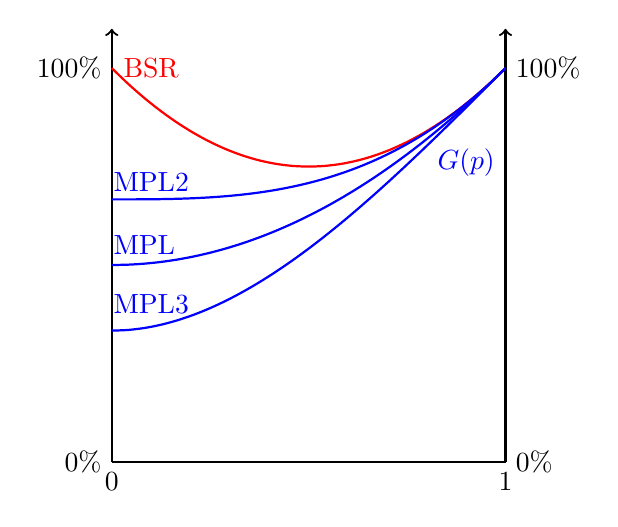
\begin{tikzpicture}[scale=5]
            \draw[thick] (0,0) node[anchor=north]{0} -- (1,0) node[anchor=north]{1};
            \draw[thick,->] (0,0) node[anchor=east]{0\%} -- (0,1) node[anchor=east]{100\%} -- (0,1.1);
            \draw[thick,->] (1,0) node[anchor=west]{0\%} -- (1,1) node[anchor=west]{100\%} -- (1,1.1);
            \draw[blue,domain=0:1, smooth, variable=\x, style={thick}]  plot ({\x}, {(1/2)*(1+ \x*\x});
            \node[blue] at (0.1,0.55) {MPL\phantom{0}};
            \draw[red,domain=0:1, smooth, variable=\x, style={thick}]  plot ({\x}, {(1/2)*(\x*\x+(1-\x)*(1-\x))+(1/2)});
            \node[red] at (0.1,1) {BSR};
            \onslide<2->{\draw[blue,domain=0:1, smooth, variable=\x, style={thick}]  plot ({\x}, {(1/3)*(2+\x*\x*\x});
            \node[blue] at (0.1,0.71) {MPL2};};
            \onslide<3->{\draw[blue,domain=0:1, smooth, variable=\x, style={thick}]  plot ({\x}, {(1/3)*(1+3*\x*\x - \x*\x*\x)});
            \node[blue] at (0.1,0.40) {MPL3};};
            \node[blue] at (0.9,0.76) {$G(p)$};
        \end{tikzpicture}\br
        \only<1-3>{\textbf{Proposition:} $G(p)$ can be made into an MPL if and only if}
        \only<4->{What's the difference across MPLs?}\\
        \only<1-3>{1. $G'(0)=0$ \hspace{1cm} 2. $G'(1)=1$ \hspace{1cm} 3. $G(1)=1$}
        \only<4>{Varying probability of rows being chosen}
    \end{center}
\end{frame}

\begin{frame}{Superiority of MPLs}
We can argue that the MPLs are superior to the BQSRs:
\br
\textbf{Theorem:}
\begin{center}
    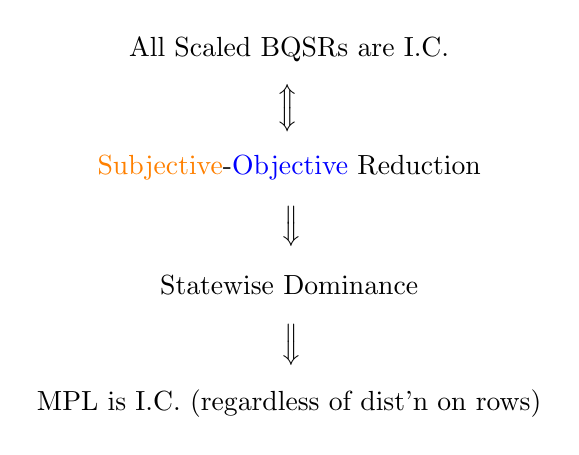
\begin{tikzpicture}[scale=5]
        \node at (0,1) {All Scaled BQSRs are I.C.};
        \node[rotate=90] at (0,0.85) {$\iff$};
        \node at (0,0.7) {{\color{orange}Subjective}-{\color{blue}Objective} Reduction};
        \node[rotate=270] at (0,0.55) {$\implies$};
        \node at (0,0.4) {Statewise Dominance};
        \node[rotate=270] at (0,0.25) {$\implies$};
        \node at (0,0.1) {MPL is I.C. (regardless of dist'n on rows)};
    \end{tikzpicture}
\end{center}
\end{frame}

\begin{frame}{Equalizing Incentives}
    \begin{center}
        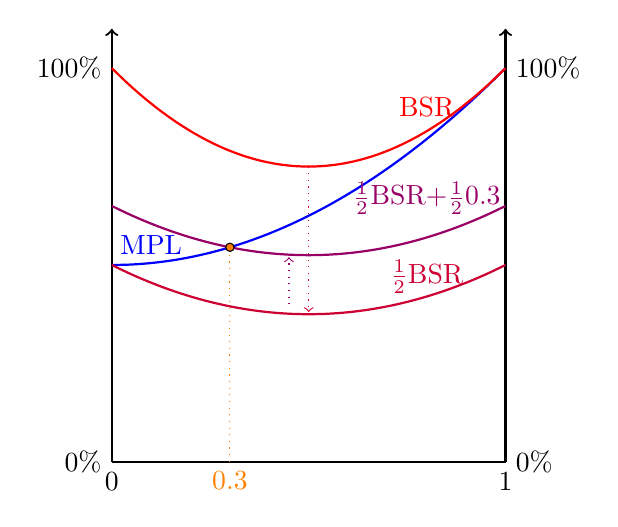
\begin{tikzpicture}[scale=5]
            \draw[thick] (0,0) node[anchor=north]{0} -- (1,0) node[anchor=north]{1};
            \draw[thick,->] (0,0) node[anchor=east]{0\%} -- (0,1) node[anchor=east]{100\%} -- (0,1.1);
            \draw[thick,->] (1,0) node[anchor=west]{0\%} -- (1,1) node[anchor=west]{100\%} -- (1,1.1);
            \draw[dotted,orange] (0.3,0) node[anchor=north]{0.3} -- (0.3,0.545);
            \draw[blue,domain=0:1, smooth, variable=\x, style={thick}]  plot ({\x}, {(1/2)*(1+ \x*\x});
            \node[blue] at (0.1,0.55) {MPL};
            \draw[red,domain=0:1, smooth, variable=\x, style={thick}]  plot ({\x}, {(1/2)*(\x*\x+(1-\x)*(1-\x))+(1/2)});
            \node[red] at (0.8,0.9) {BSR};
            \onslide<2->{\draw[red!80!blue,domain=0:1, smooth, variable=\x, style={thick}]  plot ({\x}, {(1/4)*(\x*\x+(1-\x)*(1-\x))+(1/4)+(0)*(1/2)});
            \node[red!80!blue] at (0.8,0.47) {$\frac{1}{2}$BSR};
            \draw[->,red!80!blue,dotted] (0.5,0.75) -- (0.5,0.38);};
            \onslide<3->{\draw[red!60!blue,domain=0:1, smooth, variable=\x, style={thick}]  plot ({\x}, {(1/4)*(\x*\x+(1-\x)*(1-\x))+(1/4)+(0.3)*(1/2)});
            \node[red!60!blue] at (0.8,0.67) {$\frac{1}{2}$BSR$+\frac{1}{2}0.3$};
            \draw[->,red!60!blue,dotted] (0.45,0.4) -- (0.45,0.52);};
            \filldraw[fill=orange] (0.3,0.545) circle [radius=0.3pt];
        \end{tikzpicture}\br
        How to equalize incentives across scoring rules?\\
        \only<1-2>{\textit{e.g.} suppose we know $p=0.3$}
        \only<3>{Heads: use BSR. \hspace{1cm} Tails: get \$8 w/ prob 0.3.}
    \end{center}
\end{frame}

\begin{frame}{Equalizing Incentives}
\begin{itemize}
    \item Let $X$ be r.v. representing $E$
    \begin{itemize}
        \item $\phantom{\neg}E \Rightarrow X=1$
        \item $\neg E \Rightarrow X=0$
    \end{itemize}
    \item MPL:$$S(p,x) =  \frac{1}{2}(1-(x-p)^2) + \frac{1}{2}\only<1>{x}\only<2>{{\color{red}x}}$$
    \item Suppose researcher's best guess of $p$ is $p_0$
    \item Adjusted BSR:$$S(p,x) =  \frac{1}{2}(1-(x-p)^2) + \frac{1}{2}\only<1>{p_0}\only<2>{{\color{red}p_0}}$$
\end{itemize}
\end{frame}

\begin{frame}{Other Statistics of a Distribution}
\begin{itemize}
    \item Consider again general r.v. $X$
    \begin{itemize}
        \item BSR: $S(p,x)=\left(1-(x-p)^2\right)$
    \end{itemize}
    \item Can we elicit a statistic of $p$? Ex: mean, median, mode, ...
    \item Could elicit $Pr(X=x)$ for every possible $x$... but that's a lot!
    \item The (single-report) BSR elicits the subject's \textbf{mean} for $X$
    \begin{itemize}
        \item BSR: $S({\color{blue}m},x)=\left(1-(x-{\color{blue}m})^2\right)$
        \item Still paying in probabilities
        \item Still requiring {\color{orange}S}-{\color{blue}O} Reduction:
        $$
            \max_m \sum_{{\color{orange}x}} \color{orange}Pr(X=x)\color{blue}(1-(x-m)^2)
        $$
    \end{itemize}
    \item Can we elicit the mean using an MPL?
\end{itemize}
\end{frame}

\begin{frame}{MPL for The Mean of $X$}
\begin{center}
    \only<1->{\begin{tabular}{|c|ccc|}
        \hline
        {\color{red}\textbf{Row\#}} & {\color{black!2}aaaa}{\color{red}\textbf{Option A}}{\color{black!2}aaaa} & OR & {\color{red}\textbf{Option B}} \\
        \hline
        1 & \hugme{$X$\% chance of \$8} & or & 1\% chance of \$8\\
        \hline
        2 & \hugme{$X$\% chance of \$8} & or & 2\% chance of \$8\\
        \hline
        $\vdots$ & $\vdots$ & $\vdots$ & $\vdots$\\
        \hline
        $m$ & \hugme{$X$\% chance of \$8} & or & $m$\% chance of \$8\\
        \hline
        $m$+1 & $X$\% chance of \$8 & or & \hugme{$m$+1\% chance of \$8}\\
        \hline
        $\vdots$ & $\vdots$ & $\vdots$ & $\vdots$\\
        \hline
        99 & $X$\% chance of \$8& or & \hugme{99\% chance of \$8}\\
        \hline
        100 & $X$\% chance of \$8 & or & \hugme{100\% chance of \$8}\\
        \hline
    \end{tabular}}\br
    \only<1>{Identical to two-state list: Option A is (\$8 if $E$)}
    \only<2>{Now requires linearity: ``$X$\% chance'' $\sim$ ``$E[X]$\% chance''}\\
    \only<1>{\textit{but}, now requires linearity: ``$X$\% chance'' $\sim$ ``$E[X]$\% chance''}
    \only<2>{\textit{but}, given that, IC only requires statewise dominance}
\end{center}
\end{frame}

\begin{frame}{Equalizing Incentives with Mean Elicitation}
    \begin{itemize}
        \item Researcher's best guess: mean is $\mu_0$, variance is $\sigma_0^2$
        \item (Recall: $E[X^2] = \mu_0^2 + \sigma_0^2$)
        \item BSR: $$S(p,x)=\onslide<2>{{\color{red}\frac{1}{2}}}(1-(x-m)^2)\onslide<2>{+\color{red}\frac{1}{2}(\mu_0^2 + \sigma_0^2)}$$
        \item MPL: $$S(p,x)=\frac{1}{2}(1-(x-m)^2) + \frac{1}{2}x^2$$
    \end{itemize}
\end{frame}

\begin{frame}{Eliciting the Median}
\begin{itemize}
    \item BSR elicits the mean... can we elicit the median?
    \item \textbf{Linear} scoring rule elicits the median!
    \item LSR: $$S(m,x) = (1-|x-m|) $$
    \item Can \textbf{this} be listified?
\end{itemize}
\end{frame}

\begin{frame}{MPL for The Median of $X$}
\begin{center}
    \only<1->{\begin{tabular}{|c|ccc|}
        \hline
        {\color{red}\textbf{Row\#}} & {\color{black!2}aaaa}{\color{red}\textbf{Option A}}{\color{black!2}aaaa} & OR & {\color{red}\textbf{Option B}} \\
        \hline
        1 & \hugme{\$8 if $X$ $\geq$1} & or & 50\% chance of \$8\\
        \hline
        2 & \hugme{\$8 if $X$ $\geq$2} & or & 50\% chance of \$8\\
        \hline
        $\vdots$ & $\vdots$ & $\vdots$ & $\vdots$\\
        \hline
        $m$ & \hugme{\$8 if $X$ $\geq$ $m$} & or & 50\% chance of \$8\\
        \hline
        $m$+1 & \$8 if $X$ $\geq$ $m$+1 & or & \hugme{50\% chance of \$8}\\
        \hline
        $\vdots$ & $\vdots$ & $\vdots$ & $\vdots$\\
        \hline
        99 & \$8 if $X$ $\geq$ 99 & or & \hugme{50\% chance of \$8}\\
        \hline
        100 & \$8 if $X$ $\geq$ 100 & or & \hugme{50\% chance of \$8}\\
        \hline
    \end{tabular}}\br
    Does \textit{NOT} require linearity\\
    Easily altered to elicit any quantile
\end{center}
\end{frame}

\begin{frame}{Equalizing Incentives with Median Elicitation}
    \begin{itemize}
        \item Suppose researcher's best guess of the median is $\mu_{0.5}$
        \item BSR: $$S(p,x)=\onslide<2>{{\color{red}\frac{1}{2}}}(1-|x-m|)\onslide<2>{+\color{red}\frac{1}{2}\mu_{0.5}}$$
        \item MPL: $$S(p,x)=\frac{1}{2}(1-|x-m|) + \frac{1}{2}x$$
    \end{itemize}
\end{frame}

\begin{frame}{Eliciting the Mode}
\begin{itemize}
    \item Eliciting the mode is simple \& stark:
    $$
        S(m,x) = \mathbbm{1}_{x=m}
    $$
    \item Generally: elicit most-likely interval of length $d$
    \begin{itemize}
        \item Announce any $[\underline{m},\overline{m}]$ s.t. $\overline{m}-\underline{m}=d$
        $$
            S([\underline{m},\overline{m}],x) = \mathbbm{1}_{x\in [\underline{m},\overline{m}]}
        $$
        \item Use this if $X$ has many values, since $Pr(x=m)\approx 0\ \ \forall m$
    \end{itemize}
\end{itemize}    
\end{frame}

\begin{frame}{Scoring Rules for Quantiles}
\begin{itemize}
    \item We saw MPLs can be used to elicit quantiles
    \item Scoring rule for eliciting $\alpha$ quantile (Cervera \& Mu\~{n}oz 1996):
    $$
        S(m,x) = \alpha m - (m-x)\mathbbm{1}_{x\leq m}
    $$
    \item Median is $\alpha=1/2$
    \item Proof: True distribution is $p(x)$
    \begin{align*}
        \int S(m,x) p(x) dx &= \alpha m - \int_0^m (m-x) p(x) dx \\
        FOC &: \alpha - (m-m)p(m) - \int_0^m 1\, p(x) dx = 0
    \end{align*}
    \item Announce $m$ such that $\int_0^m p(x)dx = \alpha$
\end{itemize}
    
\end{frame}

\begin{frame}{Eliciting Confidence Intervals}
\begin{itemize}
    \item We want to elicit the 95\% confidence interval
    \item Separately elicit 2.5\% quantile and 97.5\% quantile
    \item Pay one elicitation randomly
\end{itemize}
\end{frame}

\begin{frame}{The Lambert Characterization}
Lambert, Pennock \& Shoham (2008)
    \begin{itemize}
        \item In general, a \textit{statistic} is a mapping $\Gamma:\Delta(\Omega)\rightarrow \mathbb{R}$
        \item Examples: mean, median, mode, variance, kurtosis...
        \item What statistics can be elicited?
    \end{itemize}
    \textbf{Theorem:} A statistic $\Gamma$ can be elicited via a strictly proper scoring rule if and only if $\Gamma^{-1}(r)$ is a convex set of distributions for every possible statistic value $r$
\end{frame}

\begin{frame}{The Lambert Characterization}
\begin{center}
    \includegraphics[width=4in]{LectureSlides/graphics/blf/Lambert1.png}
\end{center}
Mean: yes. Variance: no!    
\end{frame}

\begin{frame}{The Lambert Characterization}
\begin{center}
    \includegraphics[width=4in]{LectureSlides/graphics/blf/Lambert2.png}
\end{center}
Median: yes!
\end{frame}

\begin{frame}{The Lambert Characterization}
\begin{center}
    \includegraphics[width=4in]{LectureSlides/graphics/blf/Lambert3.png}
\end{center}
Mode: yes!
\end{frame}

\begin{frame}{The Lambert Characterization}
\begin{center}
    \includegraphics[width=4in]{LectureSlides/graphics/blf/Lambert4.png}
\end{center}
$E[X^2]$: yes! (Why do we care?? Next slide...)
\end{frame}

\begin{frame}{The Lambert Characterization}
    \begin{itemize}
        \item We can't elicit $Var_p(X)$ with 1 report
        \item But we can elicit $E_p(X)$ and $E_p(X^2)$ 
        \begin{itemize}
            \item $Var_p(X) = E_p(X^2) - E_p(X)^2$
        \end{itemize}
        \item Or, suppose we observe two draws $X_1$ and $X_2$ from same dist'n
        \item Then $X_1-X_2$ is a new r.v.
        \item We can elicit $E_p((X_1-X_2)^2)$
            \begin{itemize}
                \item $Var_p(X) = E_p((X_1-X_2)^2)$ (check this)
            \end{itemize}
    \end{itemize}
\end{frame}

\begin{frame}{Survey of Experimental Results}
    Schotter \& Trevino (2014)\\
    Does IC matter?
    \begin{enumerate}
        \item Nelson \& Bessler (1989)
        \begin{itemize}
            \item Only use risk-neutral subjects
            \item Compare BSR to non-IC Linear SR
            \item Early periods: same. Later: differences
        \end{itemize}
        \item Palfrey \& Wang (2009)
        \begin{itemize}
            \item QSR vs LogSR vs LinearSR in games
            \item Beliefs elicited via IC mechanism are better forecasts
        \end{itemize}
    \end{enumerate}
\end{frame}

\begin{frame}{Survey of Experimental Results}
    Schotter \& Trevino (2014)\\
    Risk aversion and the standard QSR:
    \begin{enumerate}
        \item Armantier \& Treich (2013)
        \begin{itemize}
            \item Theoretical predictions for what should happen under risk aversion
            \item Observe predicted ``flatness'' in reports
            \item No incentives increases variance of reports
        \end{itemize}
        \item Offerman \& Sonnemans (2004)
        \begin{itemize}
            \item QSR performs same as flat fee
        \end{itemize}
        \item Hossain \& Okui (2013)
        \begin{itemize}
            \item BQSR outperforms QSR
        \end{itemize}
    \end{enumerate}
\end{frame}


\begin{frame}{Survey of Experimental Results}
    Schotter \& Trevino (2014)\\
    Do people best-reply to stated beliefs in games?
    \begin{enumerate}
        \item Nyarko \& Schotter (2002): yes, BR is most likely
        \item Rey-Biel (2009) 3$\times$3 games: yes, 69.4\%
        \item Blanco et al. (2011) seq. PD: yes
        \item Hyndman et al. (2013): yes, even days later
        \item Danz et al. (2012) 3$\times$3: yes
        \item Ivanov (2011): yes
        \item Manski \& Neri (2013): yes
        \item Costa-Gomes \& Weizsacker (2008)
        \begin{itemize}
            \item 14 3$\times$3 games
            \item Trt: games-then-elicitations vs. both together
            \item Can we back out beliefs from actions and match stated beliefs?
            \item Result: NO
        \end{itemize}
    \end{enumerate}
\end{frame}


\begin{frame}{Survey of Experimental Results}
    Schotter \& Trevino (2014)\\
    Does elicitation change subsequent behavior?
    \begin{enumerate}
        \item Nyarko \& Schotter (2002): no
        \item Costa-Gomes \& Weizsacker (2008): no!
        \item Ivanov (2011): no
        \item Croson (2000) VCM: yes, lower contribution
        \item Gachter \& Renner (2010) VCM: yes, higher contribution!
        \item Rutstrom \& Wilcox (2009): yes. estimated parameters of a learning model vary between QSR and no elicitation
        \item Healy (WP): mostly no
    \end{enumerate}
\end{frame}

\begin{frame}{Survey of Experimental Results}
    Schotter \& Trevino (2014)\\
    Does elicitation created hedging problems across tasks?
    \begin{enumerate}
        \item Blanco et al. (2010) seq PD: no
        \item Armantier \& Treich (2013): very little
    \end{enumerate}
\end{frame}


\begin{frame}{Healy \& Kagel}
How to test IC of belief elicitation mechanisms?\\
Problem: We need to know their true belief!
\begin{itemize}
    \item Usual technique: ``Here's a fair coin. What's Pr(H)?''
    \item Problem: too suspicious!
    \item One solution: Bayesian updating task
    \item Problem: people aren't Bayesian!
    \item Our idea: use team chat to look for evidence of conscious, intentional manipulation of reports
    \begin{itemize}
        \item Subjects are in a team of two
        \item Must submit the same belief report
        \item Chat interface to help them coordinate
        \item Do they talk about manipulating their report?
        \item Do they talk about deviating from the truth?
    \end{itemize}
\end{itemize}    
\end{frame}

\begin{frame}{Experimental Design}
    \begin{center}
        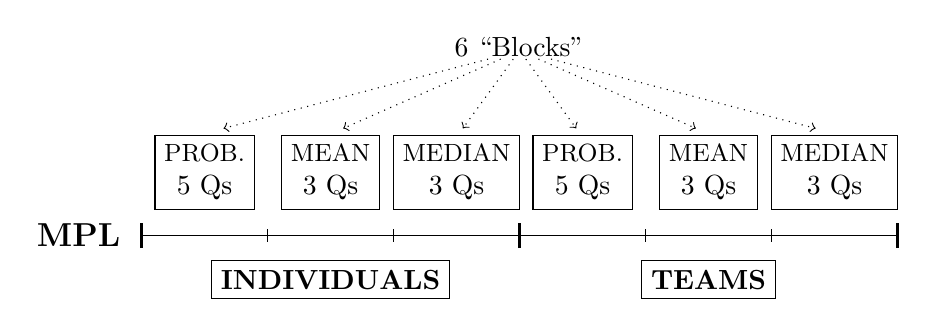
\begin{tikzpicture}[scale=0.8]
        \node[align=center] at (-1,0) {\large \textbf{MPL}};
        \draw (0,0) -- (12,0);
        \foreach \x in {0,2,...,12} {
            \draw (\x,-0.1) -- (\x,0.1);
        };
        \foreach \x in {0,6,12} {
            \draw[thick] (\x,-0.2) -- (\x,0.2);
        }
        \node[draw,align=center] at (1,1) {\small PROB.\\ 5 Qs};
        \node[draw,align=center] at (3,1) {\small MEAN\\ 3 Qs};
        \node[draw,align=center] at (5,1) {\small MEDIAN\\ 3 Qs};
        \node[draw,align=center] at (7,1) {\small PROB.\\ 5 Qs};
        \node[draw,align=center] at (9,1) {\small MEAN\\ 3 Qs};
        \node[draw,align=center] at (11,1) {\small MEDIAN\\ 3 Qs};
        \node[draw,align=center] at (3,-0.7) {\textbf{INDIVIDUALS}};
        \node[draw,align=center] at (9,-0.7) {\textbf{TEAMS}};
        \node[align=center] at (6,3) {6 ``Blocks''};
        \draw[->,dotted] (5.5,2.8) -- (1.3,1.7);
        \draw[->,dotted] (5.7,2.8) -- (3.2,1.7);
        \draw[->,dotted] (5.9,2.8) -- (5.1,1.7);
        \draw[->,dotted] (6.1,2.8) -- (6.9,1.7);
        \draw[->,dotted] (6.3,2.8) -- (8.8,1.7);
        \draw[->,dotted] (6.5,2.8) -- (10.7,1.7);
        \end{tikzpicture}\br
    \end{center}
    \begin{itemize}
        \item Each block has 3 or 5 questions of the same type
        \item Instructions before each block
        \item Order of blocks randomized within INDIV and TEAM
        \item Order of questions randomized within each block
        \item Three mechanisms: \textbf{MPL}, \textbf{BQSR}, \textbf{NoInfo}
        \begin{itemize}
            \item Each subject sees only one mechanism
        \end{itemize}
        \item INDIV first vs TEAMS first: no difference
    \end{itemize}
\end{frame}

{
\setbeamercolor{background canvas}{bg=white}
 \begin{frame}{The 11 Questions}
 \begin{center}
     \foreach \x in {1,...,11} {
         \only<\x>{\includegraphics[scale=0.4]{LectureSlides/graphics/blf/screens/a\x}\br}
         \only<\x>{\includegraphics[scale=0.5]{LectureSlides/graphics/blf/screens/b\x}}
     }
 \end{center}    
 \end{frame}

\begin{frame}{How To Present the Mechanisms}
\begin{center}
    \begin{tabular}{p{3.95in}}
    \textit{``In the first place, the subject must understand the scoring rule... This is an important reason to present the rule through some {\color{red!60!blue}vivid tabular or graphic device}...''}\\
    \multicolumn{1}{r}{--Savage (1971)}
    \end{tabular}
\end{center}\br
\br\br
\begin{itemize}
    \item \textbf{BSR:} Wilson \& Vespa (2019), Danz, Wilson \& Vesterlund (2022)
    \item \textbf{MPL:} Holt \& Smith (2016), Healy (2018)
\end{itemize}
\end{frame}

\begin{frame}{The Mechanism Interfaces: \only<1>{MPL}\only<2>{BSR}\only<3>{NoInfo}}
\begin{center}
    \only<1>{\includegraphics[scale=0.5]{LectureSlides/graphics/blf/MPL.jpg}}
    \only<2>{\includegraphics[scale=0.4]{LectureSlides/graphics/blf/QSR.jpg}}
    \only<3>{\includegraphics[scale=0.5]{LectureSlides/graphics/blf/NoInfo.jpg}}\br
    {\tiny \only<1>{\href{https://healy.econ.ohio-state.edu/exp/mpl/viewscreens.php?trt=MPL&problem=TEAM_PROB|3|3|5}{Link}}\only<2>{\href{https://healy.econ.ohio-state.edu/exp/mpl/viewscreens.php?trt=BQSR&problem=TEAM_PROB|3|3|5}{Link}}\only<3>{\href{https://healy.econ.ohio-state.edu/exp/mpl/viewscreens.php?trt=JUSTIC&problem=TEAM_PROB|3|3|5}{Link}}}
    \br
    \textbf{Note:} subjects saw the same phrase in all three treatments
\end{center}
\end{frame}

\begin{frame}{Teams Interface}
\begin{center}
    \includegraphics[scale=0.5]{LectureSlides/graphics/blf/LockIn.jpg}\includegraphics[scale=0.3]{LectureSlides/graphics/blf/Chat.jpg}\br
    \begin{itemize}
        \item Use chat window to communicate
        \item Must lock in the same number to proceed
        \item Can unlock \& change $\Rightarrow$ ``Silent agreement''
        \item If time runs out, one choice is randomly used
    \end{itemize}
\end{center}
\end{frame}
}

\begin{frame}{Logistics}
\begin{itemize}
    \item Usual OSU subject pool (ORSEE)
    \item Zoom meeting
    \item Less control of software environment $\Rightarrow$ missing observations\\
    \begin{itemize}
        \item INDIV: 1.7\% \hspace{0.3in} TEAM: 8.3\%
    \end{itemize}
    \item Venmo payments (option for in-person)
    \item \$12 show-up + possible \$8 ``bonus.'' (59\% won the bonus)
\end{itemize}\br
\begin{center}
    \# Subjects:\\
    \begin{tabular}{|r|c|c|c|}
        \hline
        Mechanism: & \textbf{MPL} & \textbf{BSR} & \textbf{NoInfo} \\
        \hline
        INDIV First: & 68 & 68 & 63 \\
        \hline
        TEAMS First: & 54 & 54 & 0 \\
        \hline \hline
        Pooled: & 122 & 122 & 63 \\
         \hline
    \end{tabular}
\end{center}
\end{frame}


{
\setbeamercolor{background canvas}{bg=white}
\begin{frame}{Objective-Easy \#1: \% Correct}
    \begin{center}
        \begin{tabular}{ m{4cm} m{4cm}}
            \includegraphics[width=1.5in]{LectureSlides/graphics/blf/urn.jpg} & {\color{purple}Pr(Red) = \uline{12/20 = 60\%}}
        \end{tabular}\br
        \% Correct:\br
        \begin{tabular}{rccc}
            & \textbf{MPL} & \textbf{BSR} & \textbf{NoInfo}  \\
            \textbf{INDIV:} & 91.7\% & 96.6\% & 92.1\% \\
            \textbf{TEAM:} & 94.8\% & 100\% & 96.4\%
        \end{tabular}
        \br
        MPL seems a little worse. Are they trying to manipulate?
    \end{center}
\end{frame}
}

\begin{frame}{Objective-Easy \#1: Chats}
    \begin{center}
        \begin{tabular}{|lcr|}
            \topchat{MPL}{181}{187}
            \leftchat{i have 12 for red}
            \leftchat{and 8 for blue}
            \rightchat{12, 20, and 75\%?}
            \rightchat{yes}
            \leftchat{75 sounds good with me}
            \answers{12|20|75\%}{12|20|75\%}
        \end{tabular}\br
        \begin{tabular}{|lcr|}
            \topchat{MPL}{289}{295}
            \leftchat{sorry I put wrong answer for 3}
            \answers{12|20|50\%}{12|20|50\%}
        \end{tabular}
    \end{center}
\end{frame}

{
\setbeamercolor{background canvas}{bg=white}
\begin{frame}{Objective-Easy \#2: \% Correct}
    \begin{center}
        \begin{tabular}{ m{4cm} m{3cm}}
            \includegraphics[width=1.5in]{LectureSlides/graphics/blf/twojarsempty.jpg} & {\color{purple}Pr(Red) = \uline{50\%}}
        \end{tabular}\br
        \% Correct:\br
        \begin{tabular}{rccc}
            & \textbf{MPL} & \textbf{BSR} & \textbf{NoInfo}  \\
            \textbf{INDIV:} & 91.5\% & 84.8\% & 93.7\% \\
            \textbf{TEAM:} & 98.3\% & 93.1\% & 100\%
        \end{tabular}\br
        Now BSR seems a little worse?
    \end{center}
\end{frame}
}

\begin{frame}{Objective-Easy \#2: Chats}
    \begin{center}
        \begin{tabular}{|p{0.7in}cr|}
            \topchat{MPL}{390}{391}
            \rightchat{50\%}
            \leftchat{so theoretically it's 50 right but i think i said 48 last time just}
            \leftchat{bc I'm in stats rn and we just did probability stuff about}
            \leftchat{how smaller sample sizes are further from the probability}
            \leftchat{so flipping it once might be 60-40 but 100 times is closer}
            \leftchat{to 50-50}
            \leftchat{but ya I'm good w just 50}
            \rightchat{makes sense}
            \rightchat{should we do 49\%}
            \leftchat{sure}
            \answers{49\%}{49\%}
        \end{tabular}\br
    \end{center}
\end{frame}

\begin{frame}{Objective-Easy \#2: Chats}
    \begin{center}
        \begin{tabular}{|p{0.7in}cr|}
            \topchat{BSR}{257}{260}
            \rightchat{50 ?}
            \leftchat{id say 60}
            \rightchat{Why}
            \leftchat{cause heads is always more likely}
            \rightchat{Thats just false}
            \leftchat{55 is a compromise}
            \rightchat{Which is also wrong but whatever}
            \answers{55\%}{55\%}
        \end{tabular}\br
        \begin{tabular}{|lcr|}
            \topchat{BSR}{357}{365}
            \multicolumn{3}{|c|}{(no chat)}\\
            \answers{75\%}{75\%}
        \end{tabular}
    \end{center}
\end{frame}



{
\setbeamercolor{background canvas}{bg=white}
\begin{frame}{Objective-Easy \#3: \% Correct}
    \begin{center}
        \begin{tabular}{ m{4cm} m{3cm}}
            \includegraphics[width=1.5in]{LectureSlides/graphics/blf/spin3.jpg} & {\color{purple} Median = \uline{60pts}}
        \end{tabular}\br
        \% Correct:\br
        \begin{tabular}{rccc}
            & \textbf{MPL} & \textbf{BSR} & \textbf{NoInfo}  \\
            \textbf{INDIV:} & 69.2\% & 83.9\% & 74.2\% \\
            \textbf{TEAM:} & 74.6\% & 86.1\% & 92.6\%
        \end{tabular}
    \end{center}
\end{frame}
}

\begin{frame}{Objective-Easy \#3: Chats}
    \begin{center}
        \begin{tabular}{|p{1.3in}cr|}
            \topchat{MPL}{343}{345}
            \leftchat{well if it was 100, 0 and 50 the median would be 50}
            \leftchat{but its 60 and so id go w like 55?}
            \rightchat{yeah}
            \answers{55\%}{55\%}
        \end{tabular}\br
        \begin{tabular}{|lcr|}
            \topchat{MPL}{352}{353}
            \rightchat{I did 60}
            \leftchat{55}
            \rightchat{55 is good}
            \answers{55\%}{55\%}
        \end{tabular}
    \end{center}
\end{frame}

\begin{frame}{Objective-Easy \#3: Chats}
    \begin{center}
        \begin{tabular}{|p{1.3in}cr|}
            \topchat{BSR}{197}{202}
            \rightchat{what do u think}
            \leftchat{hmm i don't remember what i said but maybe like 75?}
            \leftchat{i'm not sure at all}
            \rightchat{love it}
            \answers{75\%}{75\%}
        \end{tabular}\br
        \begin{tabular}{|lcr|}
            \topchat{BSR}{302}{308}
            \leftchat{80?}
            \rightchat{yeah}
            \answers{80\%}{80\%}
        \end{tabular}
    \end{center}
\end{frame}

% \begin{frame}{Objective-Hard \#1: \% Correct}
%     \begin{center}
%         \begin{tabular}{ m{4cm} m{3cm}}
%             \includegraphics[width=1.5in]{LectureSlides/graphics/blf/spin3.jpg} & {\color{purple} Mean = \uline{55pts}}
%         \end{tabular}\br
%         \% Correct:\br
%         \begin{tabular}{rccc}
%             & \textbf{MPL} & \textbf{BSR} & \textbf{NoInfo}  \\
%             \textbf{INDIV:} & 56.9\% & 46.2\% & 72.3\% \\
%             \textbf{TEAM:} & 63.6\% & 64.0\% & 90.9\%
%         \end{tabular}
%     \end{center}
% \end{frame}

% \begin{frame}{Objective-Hard \#1: Chats}
%     \begin{center}
%         \begin{tabular}{|p{1in}cr|}
%             \topchat{MPL}{181}{187}
%             \rightchat{the mean is 50 but i think we should do 60}
%             \leftchat{sound good with me}
%             \leftchat{i going to say 60 lol}
%             \answers{60\%}{60\%}
%         \end{tabular}\\
%         First evidence of deviating from belief!\br
%         \begin{tabular}{|p{0.7in}cr|}
%             \topchat{MPL}{286}{294}
%             \leftchat{55?}
%             \rightchat{i got 50}
%             \leftchat{ope you rright}
%             \rightchat{how did you do the calculation}
%             \rightchat{oh ok}
%             \answers{50\%}{50\%}
%         \end{tabular}
%     \end{center}
% \end{frame}

% \begin{frame}{Objective-Hard \#1: Chats}
%     \begin{center}
%         \begin{tabular}{|p{0.5in}cr|}
%             \topchat{BSR}{255}{263}
%             \leftchat{55}
%             \rightchat{i think}
%             \rightchat{we can only choose from}
%             \rightchat{0 60 100}
%             \leftchat{60 then?}
%             \rightchat{yeah}
%             \answers{60\%}{60\%}
%         \end{tabular}\br
%         \begin{tabular}{|p{0.7in}cr|}
%             \topchat{BSR}{304}{309}
%             \leftchat{60 is fine}
%             \answers{60\%}{60\%}
%         \end{tabular}
%     \end{center}
% \end{frame}

% \begin{frame}{Objective-Hard \#3: \% Correct}
%     \begin{center}
%         \begin{tabular}{ m{4cm} m{3cm}}
%             \includegraphics[width=1.5in]{LectureSlides/graphics/blf/spin6.jpg} & {\color{purple} Median = \uline{70pts}}
%         \end{tabular}\br
%         \% Correct:\br
%         \begin{tabular}{rccc}
%             & \textbf{MPL} & \textbf{BSR} & \textbf{NoInfo}  \\
%             \textbf{INDIV:} & 42.2\% & 51.5\% & 35.5\% \\
%             \textbf{TEAM:} & 50.9\% & 61.5\% & 53.7\%
%         \end{tabular}
%     \end{center}
% \end{frame}

% \begin{frame}{Objective-Very Hard \#4: \% Correct}
%     \begin{center}
%         \begin{tabular}{ m{4cm} m{3cm}}
%             \includegraphics[width=1.5in]{LectureSlides/graphics/blf/spin6.jpg} & {\color{purple} Mean $\approx$ \uline{55.2pts?}}
%         \end{tabular}\br
%         \% Correct:\br
%         \begin{tabular}{rccc}
%             & \textbf{MPL} & \textbf{BSR} & \textbf{NoInfo}  \\
%             \textbf{INDIV:} & 9.8\% & 5.8\% & 2.1\% \\
%             \textbf{TEAM:} & 20.8\% & 0\% & 4.6\%
%         \end{tabular}
%     \end{center}
% \end{frame}

% \begin{frame}{Objective-Hard \#5: \% Correct}
%     \begin{center}
%         \begin{tabular}{ m{4cm} m{3cm}}
%             \includegraphics[width=1.5in]{LectureSlides/graphics/blf/twojars.jpg} & {\color{purple} Pr(Red) = \uline{1/3}}\\
%             A {\color{blue} BLUE} marble was drawn & 
%         \end{tabular}\br
%         \% Correct:\br
%         \begin{tabular}{rccc}
%             & \textbf{MPL} & \textbf{BSR} & \textbf{NoInfo}  \\
%             \textbf{INDIV:} & 38.0\% & 32.7\% & 25.5\% \\
%             \textbf{TEAM:} & 55.6\% & 38.5\% & 25.0\%
%         \end{tabular}
%     \end{center}
% \end{frame}

% \begin{frame}{Objective-Hard \#5: \% Correct}
%     \begin{center}
%         \begin{tabular}{ m{4cm} m{3cm}}
%             \includegraphics[width=1.5in]{LectureSlides/graphics/blf/twojars.jpg} & {\color{purple} Pr(Red) = \uline{1/5}}\\
%             \multicolumn{2}{l}{TWO {\color{blue} BLUE} marbles were drawn} 
%         \end{tabular}\br
%         \% Correct:\br
%         \begin{tabular}{rccc}
%             & \textbf{MPL} & \textbf{BSR} & \textbf{NoInfo}  \\
%             \textbf{INDIV:} & 2.0\% & 9.6\% & 0\% \\
%             \textbf{TEAM:} & 4.3\% & 12.0\% & 0\%
%         \end{tabular}
%     \end{center}
% \end{frame}

{
\setbeamercolor{background canvas}{bg=white}
\begin{frame}{Absolute Error by Treatment}
\begin{center}
    \includegraphics[width=11cm]{LectureSlides/graphics/blf/errbydiff.png}
\end{center}
\end{frame}
}

% \begin{frame}{Order Effects?}
% \begin{itemize}
%     \item Hypothesis: They learned not to manipulate in INDIV blocks
%     \item New sessions: ``Teams First''
%     \begin{itemize}
%         \item MPL: $n=22$
%         \item BQSR: $n=26$
%         \item NoInfo: $n=0$
%     \end{itemize}
%     \item Result: Even less misreporting on Easy questions
% \end{itemize}
    
% \end{frame}

\begin{frame}{Chat Encoding}
    Two Types of Evidence of IC Failures:
    \begin{description}
        \item[Calculate] Playing with the calculator
        \begin{itemize}
            \item May not end up deviating from their belief
        \end{itemize}
        \item[Deviate] Deviate from stated belief
        \begin{itemize}
            \item May not specify \textit{why} they're deviating
        \end{itemize}
    \end{description}\br
    \only<1>{Two independent chat encoders}
    \only<2>{\begin{center}
        Team-level data:\\
        \begin{tabular}{r|ccc}
            Mechanism: & MPL & BSR & NoInfo \\
            \hline
            Calculate & 1 & 10 & 0 \\
            Deviate & 1 & 1 & 0 \\
            \hline
            Both & 0 & 1 & 0 \\
            \hline
        \end{tabular}
    \end{center}}
    \only<3>{\begin{center}
        Question-level data:\\
        \begin{tabular}{r|ccc|ccc|c}
            Mechanism: & \multicolumn{3}{c|}{\textbf{MPL}} & \multicolumn{3}{c|}{\textbf{BSR}} & \textbf{NoInfo} \\
            Question: & Obj-E & Obj-H & Subj & Obj-E & Obj-H & Subj & All \\
            \hline
            Calculate & 0 & 0 & 1 & 1 & 4 & 10 & 0 \\
            Deviate & 1 & 0 & 0 & 0 & 0 & 1 & 0 \\
            \hline
            Both & 0 & 0 & 0 & 0 & 0 & 1 & 0 \\
            \hline
        \end{tabular}\\
            Subjects use the BSR calculator when clueless!
    \end{center}}
\end{frame}


\begin{frame}{Calculate \& Deviate: BSR}
    \begin{center}
        Capital of Australia\\
        \begin{tabular}{|p{1.1in}cr|}
            \topchat{BSR}{591}{599}
            \leftchat{i said 90 bc Carnegie is a prestigious school and theyre}
            \leftchat{smart kiddos so they hv to know this easy answer}
            \leftchat{what do u think}
            \leftchat{should we go higher than 90}
            \rightchat{I think we should go higher}
            \leftchat{95/ 100?}
            \leftchat{95? 100? **}
            \rightchat{seems 100 gets the higher probability}
            \leftchat{yea with 55.9}
            \rightchat{**highest}
            \rightchat{should we do 100}
            \leftchat{yes}
            \answers{100}{100}
        \end{tabular}
    \end{center}
\end{frame}



\begin{frame}{Deviate: MPL}
    \begin{center}
         Mean of Easy Spinner\\
         \begin{tabular}{|p{1.1in}cr|}
             \topchat{MPL}{181}{187}
             \rightchat{the mean is 50 but i think we should do 60}
             \leftchat{sound good with me}
             \leftchat{i going say 60 lol}
             \answers{60}{60}
         \end{tabular}
        %  \br
        % $12/20 = 60\%$ (not flagged)\\
        % \begin{tabular}{|p{1.7in}cr|}
        %      \topchat{MPL}{352}{353}
        %      \rightchat{60\%}
        %      \leftchat{12 red marbles, 20 total, so 60\%}
        %      \rightchat{Yea but I am thinking should we really put the correct number}
        %      \rightchat{for probability}
        %      \leftchat{I mean yeah i think}
        %      \leftchat{Although its random, its the best ``odds'' then}
        %      \rightchat{alright}
        %      \answers{60\%}{60\%}
        %  \end{tabular}
    \end{center}
\end{frame}


% \begin{frame}{Deviations: BSR}
%     \begin{center}
%         Mean of Hard Quiz Score\\
%         \begin{tabular}{|p{1.1in}cr|}
%             \topchat{BSR}{305}{306}
%             \leftchat{i have no idea for this one}
%             \rightchat{i was just about to say that}
%             \leftchat{but i think 50 gives us the best shot}
%             \leftchat{just being right in the middle}
%             \rightchat{works for me}
%             \answers{50}{50}
%         \end{tabular}
%     \end{center}
% \end{frame}


\begin{frame}{Not Flagged: MPL}
    \begin{center}
        12/20/60\%\\
        \begin{tabular}{|p{1.7in}cr|}
            \topchat{MPL}{352}{353}
            \rightchat{60\%}
            \leftchat{12 red marbles, 20 total, so 60\%}
            \rightchat{Yea but I am thinking should we really put the correct number}
            \rightchat{for probability}
            \leftchat{I mean yeah i think}
            \leftchat{Although its random, its the best ``odds'' then}
            \rightchat{alright}
            \answers{60\%}{60\%}
        \end{tabular}
    \end{center}
\end{frame}

\begin{frame}{Calculate: BSR}
    \begin{center}
        Capital of Australia\\
        \begin{tabular}{|p{1.1in}cr|}
            \topchat{BSR}{407}{414}
            \leftchat{hi}
            \rightchat{hi}
            \rightchat{i noticed that the higher you make their percentage,}
            \rightchat{the higher our probability percentage gets}
            \leftchat{yeah that's true}
            \rightchat{but the closer to 50, the more equal the probs}
            \leftchat{i say we go for a big one}
            \answers{85}{85}
        \end{tabular}
    \end{center}
\end{frame}

\begin{frame}{Calculate: BSR}
    \begin{center}
        % Mean of Hard Quiz Score\\
        % \begin{tabular}{|p{0.8in}cr|}
        %     \topchat{BSR}{305}{306}
        %     \leftchat{i have no idea for this one}
        %     \rightchat{i was just about to say that}
        %     \leftchat{but i think 50 gives us the best shot}
        %     \leftchat{just being right in the middle}
        %     \rightchat{works for me}
        %     \answers{50}{50}
        % \end{tabular}\br
        Mean of Hard Quiz Score
        \begin{tabular}{|p{1.6in}cr|}
            \topchat{BSR}{298}{312}
            \rightchat{it sounds like 50 but if i took this test i might get 3/4 right}
            \leftchat{it looks like pretty much any number i type in i get 51/5\%}
            \leftchat{50 is fine ig}
            \rightchat{its the same no matter what we type is what ive seen}
            \answers{50}{50}
        \end{tabular}\\
        ($X=M \Rightarrow 51.5\%$)
    \end{center}
\end{frame}

\begin{frame}{Calculate: BSR}
    \begin{center}
        Mean of Hard Quiz Score\\
        \begin{tabular}{|p{0.8in}cr|}
            \topchat{BSR}{299}{303}
            \rightchat{40 technically gives the best odds}
            \leftchat{ok}
            \answers{40}{40}
        \end{tabular}
    \end{center}
\end{frame}

\begin{frame}{Calculate: BSR}
    \begin{center}
        Capital of Australia
        \begin{tabular}{|p{1.6in}cr|}
            \topchat{BSR}{359}{362}
            \leftchat{this was one i wasnt sure}
            \leftchat{i originally thought a high number}
            \leftchat{i put 90\% but idk}
            \rightchat{i did 48 last time but we can jack up one of the probabilities}
            \rightchat{id do 90}
            \leftchat{Isnt it Syndey? that is pretty well known right?}
            \rightchat{because it gives us 55\% chance of getting red and yes it is sydney}
            \rightchat{everyone knows that because of finding nemo lol}
            \answers{90}{90}
        \end{tabular}\\
        (90\% $\Rightarrow$ Right: 55\%, Wrong: 15\%)
    \end{center}
\end{frame}

\begin{frame}{The Story}
\begin{itemize}
    \item NoInfo performs just as well when easy, worst when hard
    \item Chats conclude they're \textbf{not} successfully manipulating
    \begin{itemize}
        \item Maybe slightly more \textit{attempts} in BSR?
    \end{itemize}
    \item Implication: Mechanism details can be distracting \textbf{or} useful
    \begin{itemize}
        \item Easy problems: details get in the way, $\uparrow$ mistakes
        \item Harder problems: details maybe help focus, $\downarrow$ mistakes
    \end{itemize}
\end{itemize}
\end{frame}


\begin{transitionframe}
  \begin{center}{ \Huge \textcolor{white}{The Pittsburgh Paper}}\end{center}
\end{transitionframe}

{
\setbeamercolor{background canvas}{bg=white}
\begin{frame}{Danz, Vesterlund, Wilson (\textit{AER} 2022)}
\begin{center}
    Easy Task misreport \%:
    
    \includegraphics[width=2.5in]{LectureSlides/graphics/blf/DVW.jpg}
\end{center}

\begin{itemize}
    \item We had $<10\%$ at 0.5 and 0.6
    \item Why do they see misreporting \& pull-to-center???
\end{itemize}
\end{frame}
}

{
\setbeamercolor{background canvas}{bg=white}
\begin{frame}{Danz Et Al. Choice Interface}
\begin{center}
    \includegraphics[width=4.5in]{LectureSlides/graphics/blf/screens/DanzEtAl_Choice.png}
\end{center}    
\begin{itemize}
    \item Clickable slider $\Rightarrow$ inexact answers $\Rightarrow$ pull to center??
    \item True probability too small??
    \begin{itemize}
        \item Changes on every screen
        \item More susceptible to distraction by payment info?
    \end{itemize}
\end{itemize}
\end{frame}
}


{
\setbeamercolor{background canvas}{bg=white}
\begin{frame}{Our Choice Interface: NoInfo}
    \begin{center}
        \includegraphics[width=4in]{LectureSlides/graphics/blf/screens/Choice_NoInfo.png}
    \end{center}
\end{frame}
}

{
\setbeamercolor{background canvas}{bg=white}
\begin{frame}{Our Choice Interface: BQSR}
    \begin{center}
        \includegraphics[width=2in]{LectureSlides/graphics/blf/screens/Choice_BSR.png}
    \end{center}
\end{frame}
}

{
\setbeamercolor{background canvas}{bg=white}
\begin{frame}{Our Choice Interface: MPL}
    \begin{center}
        \includegraphics[width=2.7in]{LectureSlides/graphics/blf/screens/Choice_MPL.png}
    \end{center}
\end{frame}
}

\begin{frame}{Instructions Only}
``Instructions-Only'' Treatment
\br
How I would \textit{actually} do elicitation:
\begin{itemize}
    \item Mechanism details in Sinstructions
    \item No details on decision screens
\end{itemize}    
\end{frame}

\begin{frame}{Details}
    Prolific + Qualtrics\\
    US adults 18+\\
    3 comprehension Q's
    \begin{center}
        \begin{tabular}{r|cc}
             & Total $n$ & \% Pass Comp. Test \\
        \hline
        MPL  & 99 & 92\% \\
        BQSR & 99 & 86\% \\
        MPL-InstrOnly & 100 & 90\% \\
        BQSR-InstrOnly & 101 & 95\% \\
        NoInfo & 103 & 98\% \\
        \multicolumn{1}{c}{ } & \multicolumn{2}{c}{\footnotesize{$\chi^2$ test $p$-value: 0.015}}
        \end{tabular}
        
    \end{center}

\end{frame}

{
\setbeamercolor{background canvas}{bg=white}
\begin{frame}{Robust Replication Results}
    \begin{center}
        \includegraphics[width=4.4in]{LectureSlides/graphics/blf/Misreporting_Replication.png}
    \end{center}
\end{frame}
}

\begin{frame}{Differences?}
``Robust replication'' vs. ``exact replication''
\br
Differences:
\begin{enumerate}
    \item Pitt Lab adults vs. Prolific US adults
    \item Clickable slider vs. text input
    \item Different illustrations of the question
    \item We scaled BQSR to make expected payment = MPL
    \item Instructions similar, not the same
    \item Different calculator interfaces\\
    $\vdots$
\end{enumerate}    
\end{frame}

\begin{frame}{A Non-IC Mechanism}
Recall Linear Scoring Rule (LSR):
    \begin{center}
        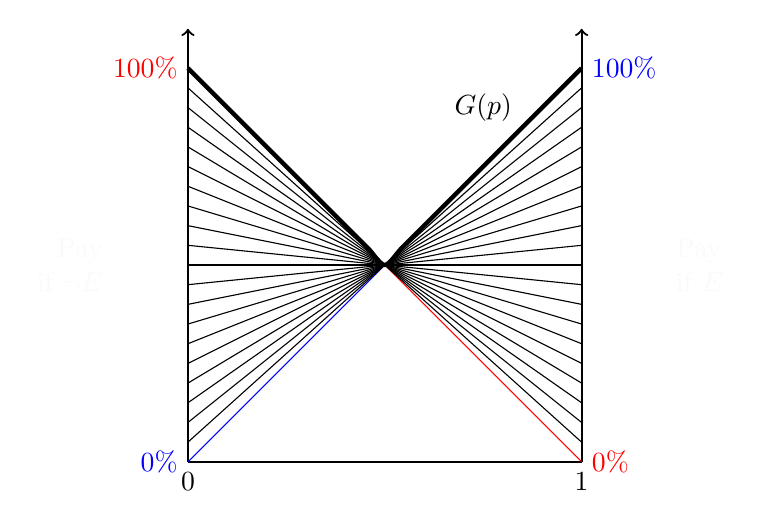
\begin{tikzpicture}[scale=5]
            \node[align=right,color=black!2] at (-0.3,0.5) {Pay\\if $\neg E$};
            \node[align=left,color=black!2] at (1.3,0.5) {Pay\\if $E$};
            \draw[thick] (0,0) node[anchor=north]{0} -- (1,0) node[anchor=north]{1};
            \draw[thick,->] (0,0) node[anchor=east]{\color{blue}0\%} -- (0,1) node[anchor=east]{\color{red}100\%} -- (0,1.1);
            \draw[thick,->] (1,0) node[anchor=west]{\color{red}0\%} -- (1,1) node[anchor=west]{\color{blue}100\%} -- (1,1.1);
            \draw[blue] (0,0) -- (1,1);
            \draw[red] (0,1) -- (1,0);
            \foreach \x in {5,10,...,95} {
                \pgfmathsetmacro\qsrl{1 - (\x/100)};
                \pgfmathsetmacro\qsrr{(\x/100)};
                \draw (0,\qsrl) -- (1,\qsrr);
            }
            \draw[domain=0:1, smooth, variable=\y, style={ultra thick}]  plot ({\y}, {max(\y,1-\y)});
            \node at (0.75,0.9) {$G(p)$};
        \end{tikzpicture}\br
        $S(q,0)=1-q$\hspace{1in}$S(q,1)=q$\\
        $q^*=0$ if $p<50$, $q^*=100$  if $p>50$
    \end{center}
\end{frame}    

\begin{frame}{A Non-IC Mechanism}
Why test this?
\begin{enumerate}
    \item Validating the chat methodology
    \begin{itemize}
        \item They \textit{should} deviate...
        \item so do we see them chat about it?
    \end{itemize}
    \item Does incentive compatibility even matter?
    \begin{itemize}
        \item Maybe they don't pay attention!
    \end{itemize}
\end{enumerate}    
\end{frame}

\begin{frame}{A Non-IC Mechanism}
Preliminary results:
\begin{itemize}
    \item Chat data:
    \begin{itemize}
        \item Out of 30+ subjects, only \textbf{one} mentions it
        \item And their partner dismisses it!
    \end{itemize}
    \item Choice data:
    \begin{itemize}
        \item INDIV: a few more cases of 100 and 0!!
        \item TEAM: no differences
    \end{itemize}
\end{itemize}
I can't get people to lie!!!\\
\textit{Really} don't replicate Danz et al. (2022)
\end{frame}

\begin{transitionframe}
    \vfill
  \begin{center}{ \Huge \textcolor{white}{Tangential Results}}\end{center}
  \vfill
\end{transitionframe}

\begin{frame}{Errors in Bayesian Updating}
\begin{center}
        \includegraphics[width=1.5in]{LectureSlides/graphics/blf/twojars.jpg}\br
\end{center}
\begin{itemize}
    \item One Blue Draw:
    \begin{itemize}
        \item $Pr(R|b) = Pr(R)*Pr(b|R)$. 17\%
        \item Marble draw is uninformative. 50\%
    \end{itemize}
    \item Two Blue Draws:
    \begin{itemize}
        \item $Pr(R|bb) = Pr(R)*Pr(b|R)*Pr(b|R)$. 6\%
        \item Second draw gives no new info. Same as one.
        \item Marble draws are uninformative. 50\%
        \item Second draw was with replacement. 0\%
    \end{itemize}
\end{itemize}
\end{frame}

{
\setbeamercolor{background canvas}{bg=white}
\begin{frame}{Does The Truth Win?}
``Truth-Wins'' Norm:
\begin{description}
    \item[2 Right:] Both players were correct in INDIV
    \item[1 Right:] One player was correct in INDIV
    \item[Team Right:] Both players correct in TEAM ($n=73$ teams)
\end{description}\br
\begin{tabular}{rccc}
     & & & Median \\
     &  \includegraphics[width=0.6in]{LectureSlides/graphics/blf/urn.jpg} & \includegraphics[width=1in]{LectureSlides/graphics/blf/twojarsempty.jpg} & \includegraphics[width=0.6in]{LectureSlides/graphics/blf/spin3.jpg} \\
      \textbf{Team Right|2 Right:} & 80/83 & 64/69 & 46/51 \\
      \color{blue}\textbf{Team Right|1 Right:} & \color{blue}8/10 & \color{blue}22/24 & \color{blue}26/34 \\
    \textbf{Team Right|0 Right:} & 0/1 & 1/1 & 1/9
\end{tabular}
\end{frame}
}

{
\setbeamercolor{background canvas}{bg=white}
\begin{frame}{Does The Truth Win?}
\begin{tabular}{rccc}
     & Mean & Median & 1 {\color{blue}BLUE} \\
     &  \includegraphics[width=0.6in]{LectureSlides/graphics/blf/spin3.jpg} & \includegraphics[width=0.6in]{LectureSlides/graphics/blf/spin6.jpg} & \includegraphics[width=1in]{LectureSlides/graphics/blf/twojars.jpg} \\
      \textbf{Team Right|2 Right:} & 26/29 & 16/21 & 7/8 \\
      \color{blue}\textbf{Team Right|1 Right:} & \color{blue}29/42 & \color{blue}24/41 & \color{blue}26/47 \\
    \textbf{Team Right|0 Right:} & 6/23 & 8/32 & 3/39
\end{tabular}
\end{frame}
}

\begin{frame}{Aggregating Beliefs}
    \begin{enumerate}
        \item Prediction Markets
            \begin{itemize}
                \item Double-auction w/ Arrow securities
            \end{itemize}
        \item Market Scoring Rules
        \item Parimutuel Betting Markets
        \item The Delphi Method
        \item Bayesian Truth Serum
    \end{enumerate}
\end{frame}

\begin{frame}{Prediction Markets}
\begin{itemize}
    \item Double auction w/ Arrow securities ($\$1$ if $E$)
    \item Wave of popularity: \citet{WolfersZitzewitz2004}
    \begin{itemize}
        \item Iowa Electronic Markets \citep{BergEtAl1996}
        \item TradeSports \& InTrade
        \item In-house markets
        \begin{itemize}
            \item Google \citep{CowgillEtAl2009}
            \item HP \citep{HoChen2007}
        \end{itemize}
        \item DARPA Policy Analysis Market \citep{Hanson2007}
    \end{itemize}
    \item Theory problem: does Walrasian equilibrium really aggregate info?
    \begin{itemize}
        \item \citet{Manski2006}: No
        \item Other models: yes (cite needed!)
    \end{itemize}
\end{itemize}
\end{frame}

\begin{frame}{Market Scoring Rules}
\cite{Hanson2003,LedyardEtAl2009}
        \begin{itemize}
            \item Start with public distribution $p_0$
            \item Player $i$ moves it to some $p_1$
            \item Paid $S(p_1,x) - S(p_0,x)$
            \item IC since $S(p_0,x)$ doesn't depend on $p_1$
            \begin{itemize}
                \item Except for dynamic incentives...
            \end{itemize}
            \item Player $i$ ``buys out'' previous player
        \end{itemize}
\end{frame}

\begin{frame}{Pari-Mutuel Betting}
    \begin{itemize}
        \item Bettor $i$ bets $b_{ij}$ on horse $j$
        \item If horse $k$ wins, bettor $i$ gets
        $$
            \underbrace{\left(\sum_{ij} b_{ij} - T\right)}_{\text{net proceeds after take $T$}} \underbrace{\frac{b_{ik}}{\sum_\iota b_{\iota k}}}_{\text{$i$'s bet share on $k$}}
        $$
        \item \citet{KoesslerEtAl2002}: fully-revealing BNE if simultaneous, not seq.
        \item Behavioral observations:
        \begin{itemize}
            \item Mirages: \citet{CamererWeigelt1991}
            \item Favorite-Longshot Bias: \citet{SnowbergWolfers2006}
            \item End-Of-Day Risk Seeking (Camerer?)
        \end{itemize}
    \end{itemize}
\end{frame}

\begin{frame}{Iterated Polls/Delphi Method}
    Simple procedure:
    \begin{enumerate}
        \item Privately ask everyone's prior
        \item Reveal all priors (or aggregate) to everyone
        \item Players update
        \item Repeat $m$ times (or until convergence)
        \item Pay everyone via scoring rule for final $p$
    \end{enumerate}
    \br
    \begin{itemize}
        \item Naive play gives info aggregation
        \item Dynamic incentives? \citet{McKelveyPage1990}
        \begin{itemize}
            \item ``Last moves'' are incentive compatible
        \end{itemize}
    \end{itemize}
\end{frame}

\begin{frame}{An Experimental Test}
\cite{HealyEtAl2010}
\begin{itemize}
    \item Compare DA, MktSR, Parimutuel, \& Poll
    \item Thin markets: $n=3$.
    \item $|\Omega|=2$ vs. $|\Omega|=8$, Traders see different \# of signals
\end{itemize}
Signal structure (common info):
\includegraphics[width=3in]{LectureSlides/graphics/blf/HealyEtAlSignalStructure.png}
\end{frame}

\begin{frame}{An Experimental Test}
Measures of Performance:
\includegraphics[width=2.8in]{LectureSlides/graphics/blf/HealyEtAlInconsistent.png}\\
1. $l_2$ distance from ``full info posterior''\\
2. Bayes-Inconsistency    
\end{frame}

\begin{frame}{An Experimental Test}
Distance to full-info posterior:\\
\begin{center}
    \includegraphics[height=2.8in]{LectureSlides/graphics/blf/HealyEtAl1.png}
\end{center}
\end{frame}

\begin{frame}{An Experimental Test}
Distance to Bayes-consistency ($|\Omega|=8$):\\
\begin{center}
    \includegraphics[width=3in]{LectureSlides/graphics/blf/HealyEtAlInconsistentResults.png}
\end{center}
\end{frame}

\begin{frame}{An Experimental Test}
Measures of Performance:
\includegraphics[width=2.8in]{LectureSlides/graphics/blf/HealyEtAlMirages.png}\\
3. Mirages\\
4. No trade!    
\end{frame}

\begin{frame}{An Experimental Test}
Mirages and No Trade ($|\Omega|=8$):\\
\begin{center}
    \includegraphics[width=4.2in]{LectureSlides/graphics/blf/HealyEtAlMiragesResults.png}
\end{center}
\end{frame}

\begin{frame}{An Experimental Test}
Summary:\\
\begin{center}
    \includegraphics[width=4.2in]{LectureSlides/graphics/blf/HealyEtAlResultsSummary.png}
\end{center}
\end{frame}

\begin{frame}{Bayesian Truth Serum}
    \cite{Prelec2004}\\
    Method to get truthful answers to a survey question.
    \begin{itemize}
        \item Agents: $i\in\{1,\ldots,n\}$.
        \item Options/answers: $j\in\{1,\ldots,m\}$
        \item Each $i$ announces:
        \begin{enumerate}
            \item their answer $t_i\in\{1,\ldots,m\}$
            \item their distribution of other's answers $p_i(\cdot)\in \Delta(\{1,\ldots,m\})$
        \end{enumerate}
        \item Define:
        \begin{itemize}
            \item $I_{ij}=1$ iff $t_i = j$
            \item $\bar{x}_j = \frac{1}{n} \sum_i I_{ij}$\\
            Actual average frequency of $j$
            \item $\bar{y}_j=\exp \left(\frac{1}{n}\sum_i \log (p_i(j)) \right)$\\
            Geometric average predicted frequency of $j$
        \end{itemize}        
    \end{itemize}
\end{frame}

\begin{frame}{Bayesian Truth Serum}
    Incentives:
    \begin{itemize}
        \item ``info score'' for each option: $\iota(j) = \log \left( \frac{\bar{x}_j}{\bar{y}_j} \right)$
        \item prediction penalty: $\rho(p_i) = \sum_{j=1}^m \bar{x}_j \log \left( \frac{p_i(j)}{\bar{x}_j} \right)$
    \end{itemize}
    Payoff:
    $$
    \pi(t_i,p_i(\cdot)) = \iota(j) + \alpha \rho(p_i)
    $$
    \textbf{Theorem:} Assume opinions ($t_i$) are exchangeable and $n$ is large. Then truth-telling is a Bayes-Nash equilibrium. Furthermore, among equilibria, it is the equilibrium that maximizes the expected info score
\end{frame}

\begin{frame}[allowframebreaks]
    \frametitle{References:}
    \small
    \bibliographystyle{plainnat}
    %\bibliographystyle{elsarticle-harv}
    \bibliography{pjzotero}
\end{frame}

\end{document}